\documentclass[12pt]{article}
\usepackage{geometry}
\geometry{letterpaper}
\usepackage{graphicx}
\usepackage{wrapfig}
\graphicspath{{/Users/benjaminbolling/Dokument/FYSB06/ANACONDA_2/Manuals/gui/Screens/}}
\begin{document}
\title{Manual for the {\it GUI\/} of {\it ANACONDA2\/}} 
\author{Benjamin Bolling,$^{1\ast}$}
\maketitle
$^{1\ast}$Department of Physics, Lund University, Lund, Sweden.

\clearpage
\section*{Abstract}
This manual will teach the user the basics of data treatment by using the GUI (Graphical User Interface) of the ANACONDA2 (ANAlysis of COiNcidence DAta) data treatment package for MATLAB.\\
\\
The GUI is divided into different tabs for different levels of data treatments, and hence, the manual is divided into the corresponding sections:

\subsection*{File Handler}
The file handler section shows how raw experimental data files are loaded and handled by the ANACONDA2 GUI's file-handler and the different operations that can be performed in this tab.

\subsection*{Data Calibration}
Raw data has to be calibrated using different calibration procedures for different types of experiments.

\subsection*{Data Filters}
Filters have to be constructed in order to filter out possible noise and uninteresting data. Multiple filters can be applied to multiple experiments, with various translate conditions. In order to let the user avoid high-level coding in order to construct multilayer data filters, a UITree JAVA-component has been inserted into the GUI in order to allow advanced filter editing procedures by simple DnD (drag-and-drop) actions. This also saves the users lots of time by eliminating the need for raw coding.

\subsection*{Plotting}
Plotting is crucial for all experiments in order to comprehend experimental data. There are various alternatives for plotting: Pre-defined and user-defined plot configurations, and the latter either with pre-defined or user-defined signal configurations.

\clearpage
\tableofcontents

\clearpage
\section{Introduction to the ANACONDA2 GUI}
\subsection*{Aim of this document}
The aim of this document is to introduce the reader to the data treatment software ANACONDA2's graphical user interface (GUI). 

\subsection*{Central concepts}
In the ANACONDA2 package, there are two layers for the users: A command-line (kernel-only) layer and a graphical layer. The graphical layer is built upon the command-line layer in order to enable users with a lack of coding (or MATLAB) experience to use the ANACONDA2 package. For the documentation of the kernel-only layer of the ANACONDA2 package, see ref. \cite{Bart_Documentation}.\\
\\
Metadata is, as described and defined by ref. \cite[chapter 2, pp.~4--6]{Bart_Documentation}, a set of information defined for each experiment which is "needed to correct, convert, fit and visualize the data". The description of the metadata structure can be found in ref. \cite[chapter 2, pp.~4--5]{Bart_Documentation}, and will not be elaborated any further in this document, since the aim of this document is, as previously described, to describe how to use the ANACONDA2 package graphically via the ANACONDA2 GUI.\\
\\
A concept that is very central to the ANACONDA2 GUI is data filters. A data filter is built upon one or a set of logical condition(s). An example of a data filter built upon one logical condition for e.g. a mass-spectrometry experiment is a 'hits-filter' that only allows hit detections of single molecular fragments (hits) which have a mass-over-charge between 20-40 Da, or an 'events-filter' which only allows events having a total mass-over-charge between 40-50 Da (where the event's mass-over-charge is the sum of the mass-over-charge of the individual hits associated with the specific event). An example of a data filter built upon a set of logical conditions is e.g. a filter which combines the previously described hit- and event filter with different translate conditions, such as 'AND' and 'OR', where 'AND' means that both conditions have to be fulfilled and 'OR' means that at least one of the conditions have to be fulfilled, in order for the data to be allowed through for e.g. plotting. This can be described as data selection, where the user defines the data points of interest such that the data-points of no interest are neglected.\\ \\�\\
\\
The filters are constructed as metadata for each experiment individually, based either on locally defined metadata and/or metadata pre-defined by the ANACONDA2's spectrometer settings (during the loading of the files). There are hard-coded built-in filters that are not connected to any experiment, which cannot be edited directly but can be added to different experiments and then edited. The filters associated with the various experiments are further on referred to as user-defined filters.\\
\\
A signal is defined as something that for every hit has a value, and it could be either raw (coming directly from a spectrometer) or have a physical quantity (e.g. mass-over-charge, kinetic energy, etc.).

\subsection*{System requirements}
- A computer which can run the latest$^*$ version of MATLAB.\\
- A licensed and verified version of MATLAB.\\
- The ANACONDA2 package.\\
\\
The following toolboxes are required:\\
Neural Network Toolbox, \\
\\
$^*$R2017a is required in this instance. Since ANACONDA2 is and will be continuously updated with new functionalities implemented from updated versions of MATLAB, the latest running version of MATLAB and ANACONDA2 is recommended in order to avoid bugs and compatibility issues.

\subsection*{Setup of ANACONDA2 and ANACONDA2 GUI}
1. Download the ANACONDA2 package to the preferred folder.\\
2. Change to or add this folder to MATLAB path.\footnote{There are two ways to change/add a folder to the MATLAB path: Graphically or by using commands. By using commands; type [ addpath 'dirname'�] and press enter (replace 'dirname' with the path of the package, e.g.: /home/user/matlab on Mac OS X). Graphically; browse into the location of the ANACONDA2 package, open the ANACONDA2 folder, right-click on the 'package' folder and select 'Add to Path' $\rightarrow$ 'Selected Folders'. Note: Do not select 'Selected Folders and Subfolders'!}.\\
3. In order to start the GUI; write [ GUI.main ] and press enter.

\clearpage
\subsection*{ANACONDA2 GUI overview}
\begin{wrapfigure}{r}{0.3\textwidth}
\centering
  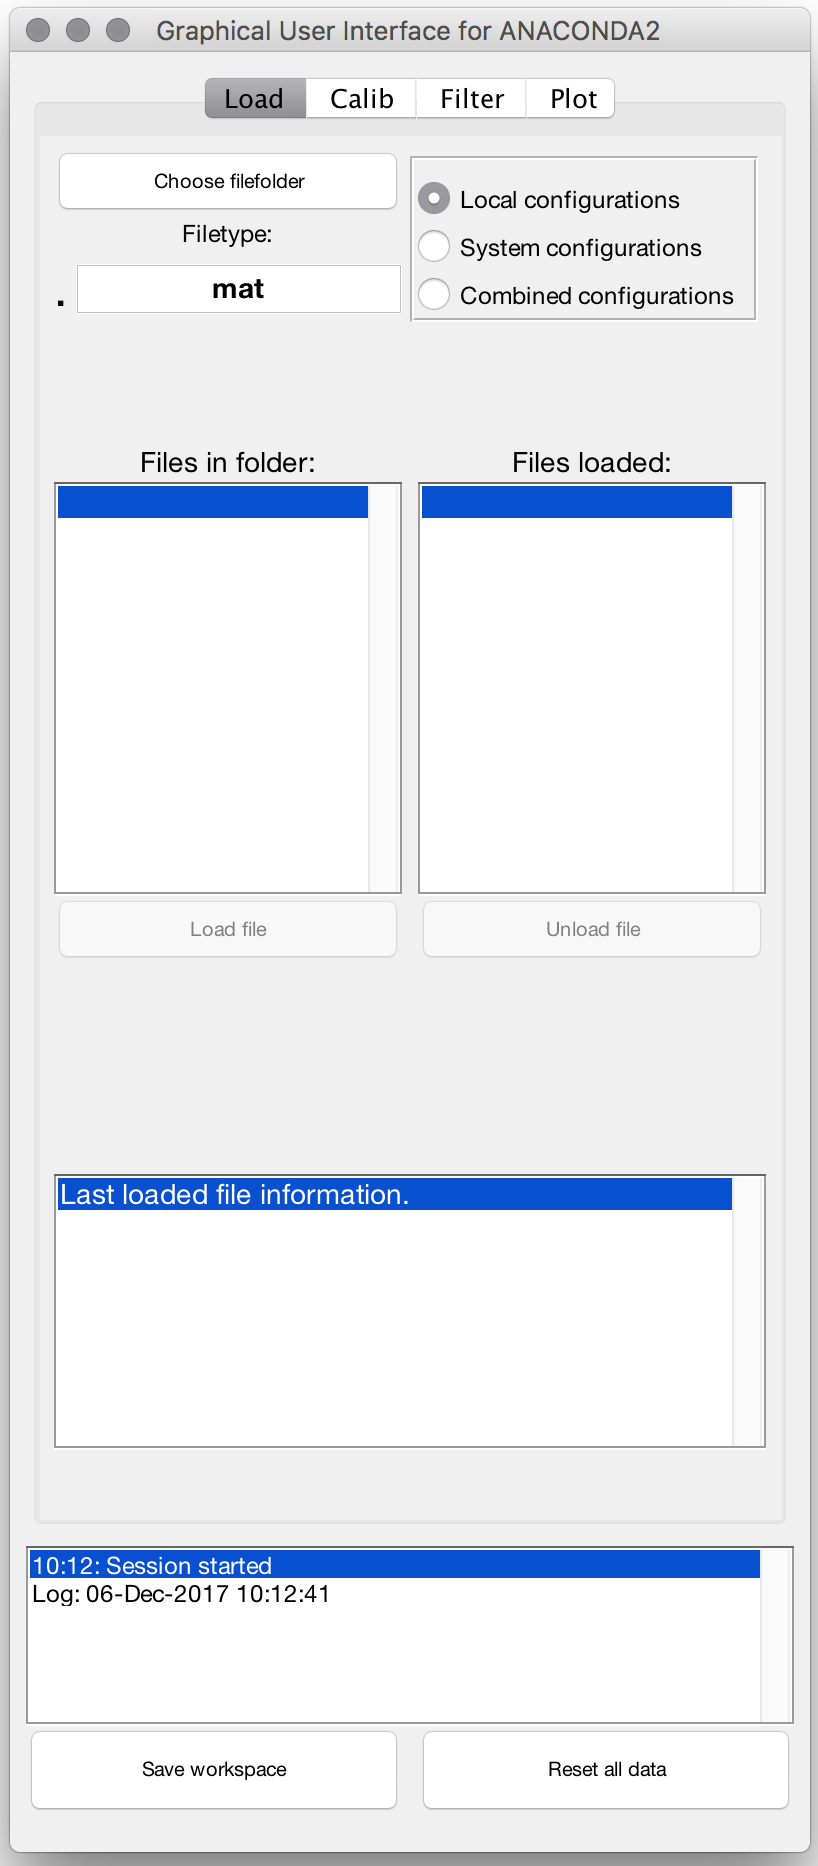
\includegraphics[width=0.3\textwidth]{1_1_startup}
 \caption{The start screen when launching the ANACONDA2 GUI.}\label{1_1_startup}
\end{wrapfigure}
When launching the ANACONDA2 GUI, the screen will look similar to Figure~\ref{1_1_startup}. There are four tabs, each representing a different part of the data treatment process in a chronological order.\\
\\
The first tab is a file handler tab, labelled as 'Load' since this is where files are loaded (resp. unloaded).\\
\\
The second tab is a calibration tab, labelled as 'Calib', where raw data files coming directly from experiments can be calibrated via multiple calibration procedures.\\
\\
The third tab is a filter tab in which data filters can be constructed, edited, removed and combined.\\
\\
The fourth tab is the plot tab, in which data can be plotted and where new plot- and signal configurations can be created.\\
\\
On the bottom, there is a big window which is the 'log box'. In it, the different actions performed with the GUI can be found.\\
\\
Reset all data means that the GUI will restart and all work will be deleted.\\
\\
Save workspace means that all files that have been loaded will have their respective metadata files replaced or stored in their respective location.

\clearpage
\section{Data treatment part 1: File Handler}
\begin{figure}[h]
\centering
  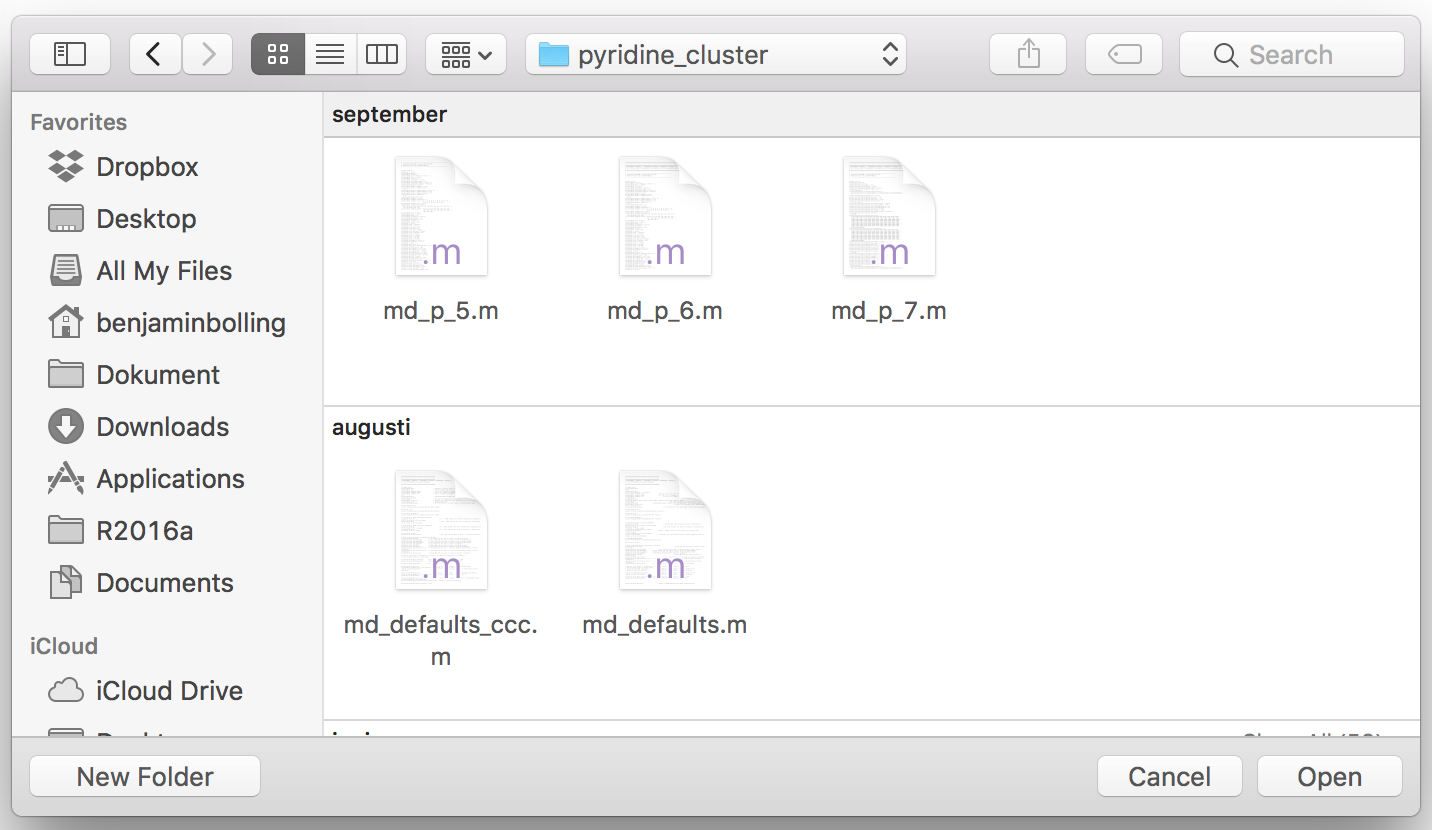
\includegraphics[width=0.4\textwidth]{1_2_choosefolder}
 \caption{Browse into the folder where the experimental data files are located.}\label{1_2_choosefolder}
\end{figure}
To load data files, they have to be in one of the following filetypes: .dlt, .mat.\\
\begin{wrapfigure}{r}{0.3\textwidth}
\centering
  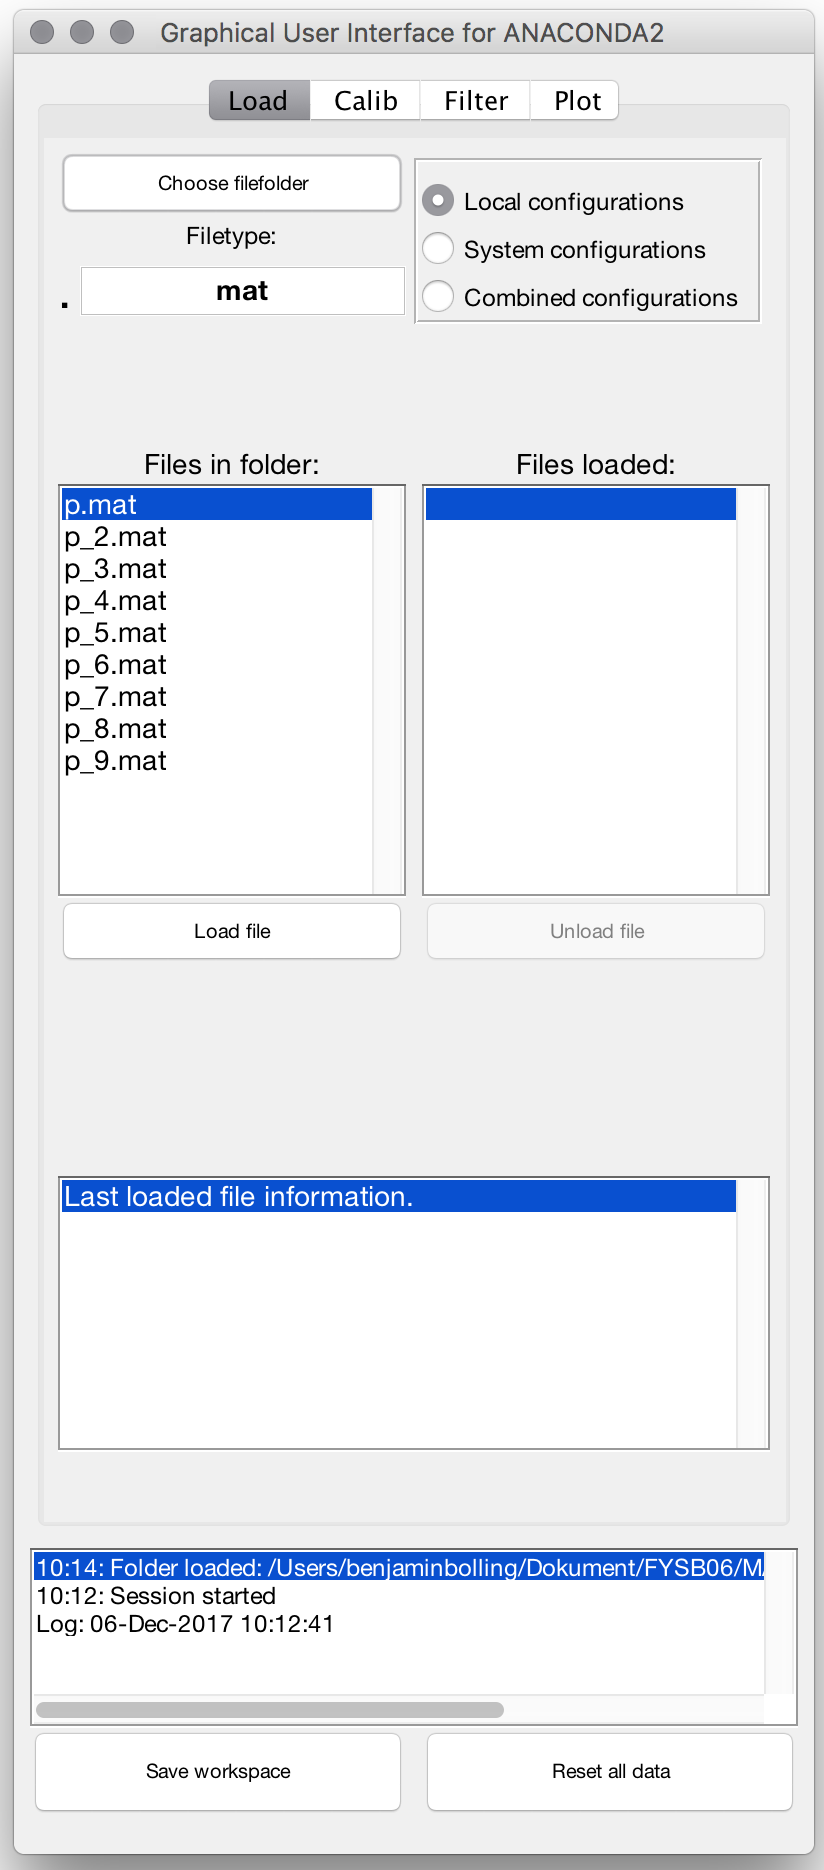
\includegraphics[width=0.3\textwidth]{1_3_choosefile}
 \caption{Files in selected folders with selected filetype can be seen.}\label{1_3_choosefile}
\end{wrapfigure}
In order to get the files from an experiment, click on 'Choose filefolder' and browse into the folder where the experimental data files are located and press 'Open'. Once opened, the filehandler will show all files with the selected file-extension (e.g. '.mat' as seen in Figure~\ref{1_3_choosefile}) in the folder. The filetype can be edited by simply clicking in the box and writing another file-extension, e.g. '.dlt', and pressing enter or with the mouse anywhere outside the box. This will result in that all '.dlt'-files in the folder will be shown.\\
Before loading a file, the load configurations should be selected which describes how a file is to be loaded.
\begin{itemize}
\item'Local configurations' selected means that if there is a readable configuration file in the same folder with the name 'md\_[filename].m', this file will be used when the [filename] data file is loaded.
\item'System configurations' means that a pre-defined spectrometer can be selected in order to generate the metadata necessary for the data treatment.
\item'Combined configurations' means that both local and system configurations will be used. If any overlap is found for a metadata, the metadata defined in local configurations will be used.
\end{itemize}
\clearpage
\begin{figure}[h]
\centering
  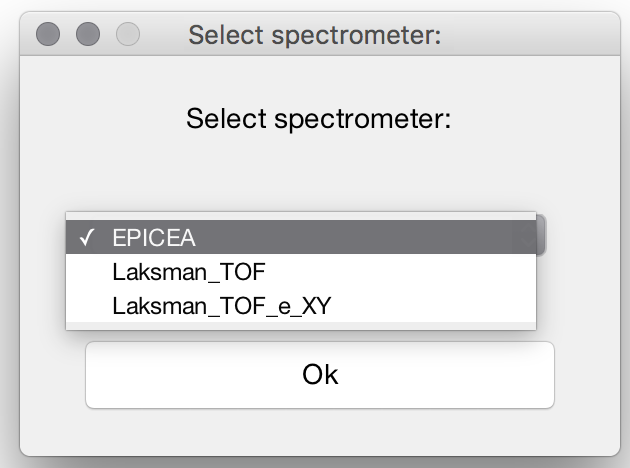
\includegraphics[width=0.4\textwidth]{1_4_loadfile_specset}
 \caption{When using system configurations to load a file, there are three spectrometers that can be chosen from.}\label{1_4_loadfile_specset}
\end{figure}
\begin{wrapfigure}{r}{0.3\textwidth}
\centering
  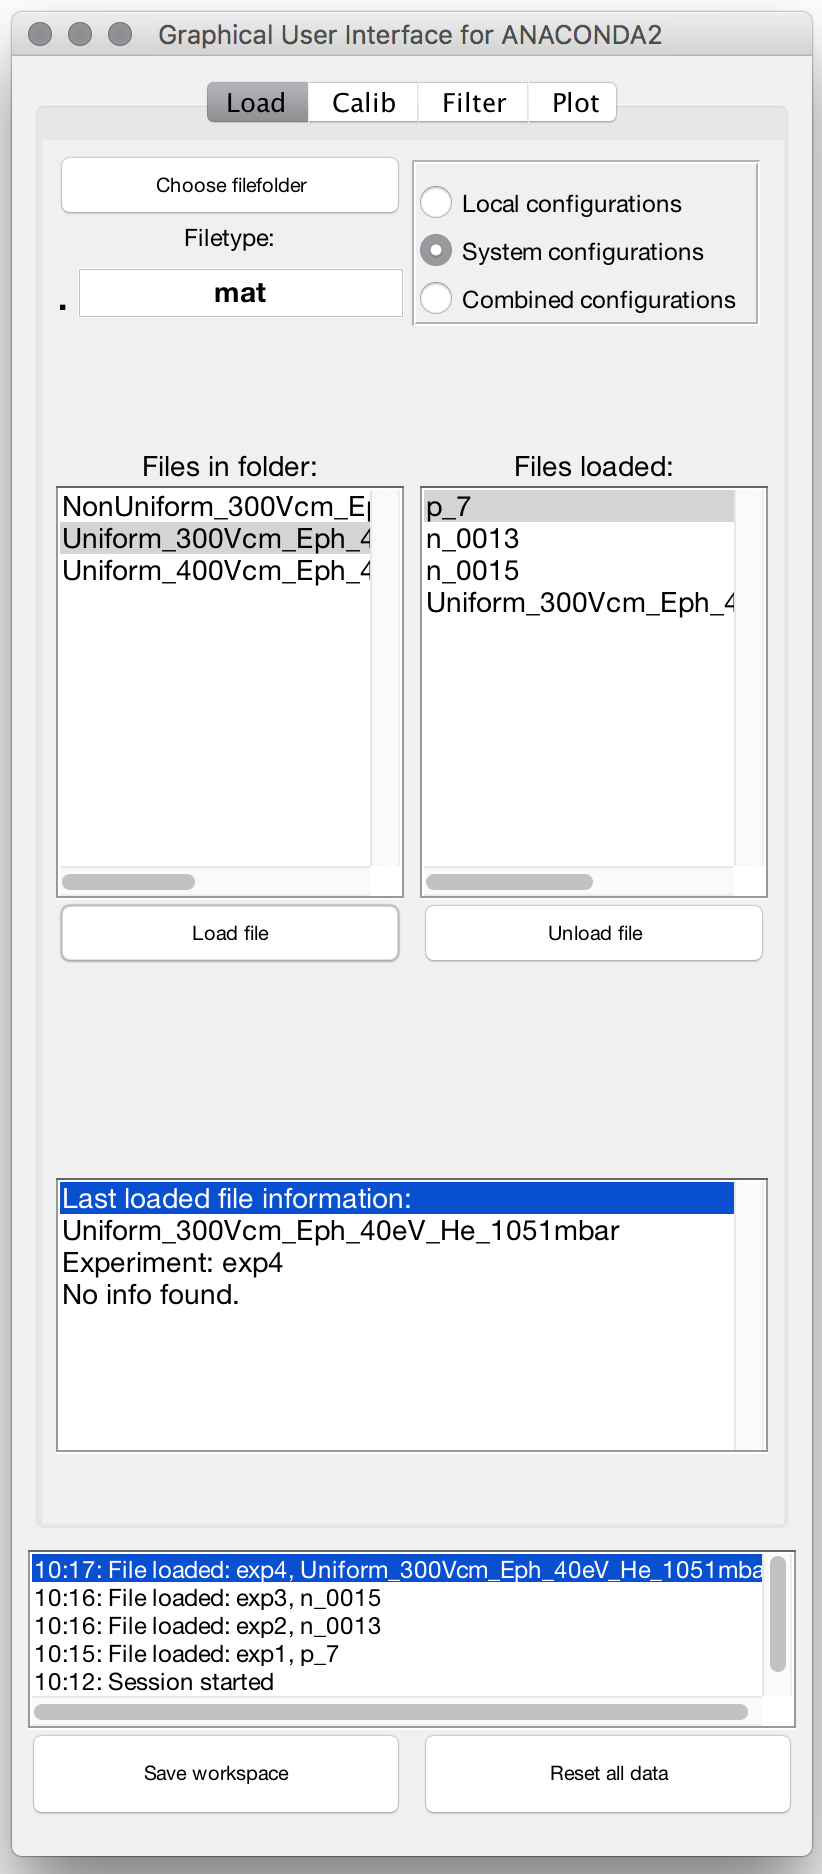
\includegraphics[width=0.3\textwidth]{1_5_filesloaded}
 \caption{Files in selected folders with selected filetype can be seen.}\label{1_5_filesloaded}
\end{wrapfigure}
There are currently three available spectrometers: EPICEA, Laksman\_TOF and Laksman\_TOF\_e\_XY. Their properties and differences can be found in the attachment 'ANACONDA2 built-in Spectrometers'.\\
\\
To load the selected file, press 'Load file' after having selected the desired configurations. As files are being loaded into memory, they will be visible in the 'Files loaded'-list. The last loaded file's information will be shown in the file information window, which exists if it has been properly defined during data acquisition during an experiment. Selecting a loaded file results in that this file's information will be shown in the file information window.\\
\\
To unload a file from memory, select a loaded file and press 'Unload file'.\\
\\
In our example, we have loaded 4 different data files from 3 different experiments, stored at three different locations. The first three files have been loaded using local configurations whilst the last file was loaded with system configurations with the Laksman\_TOF\_e\_XY spectrometer.

\clearpage
\section{Data treatment part 2: Data Calibration}
[ NOT YET CONSTRUCTED. ]

\clearpage
\section{Data treatment part 3: Data Filters}
The actions that can be done with data filters is the following: Construction of new filters, editing filters, renaming filters and removing filters. The fontsize of the filters can be increased resp. decreased by clicking on [A+] resp. [A-].
\begin{wrapfigure}{r}{0.34\textwidth}
\centering
  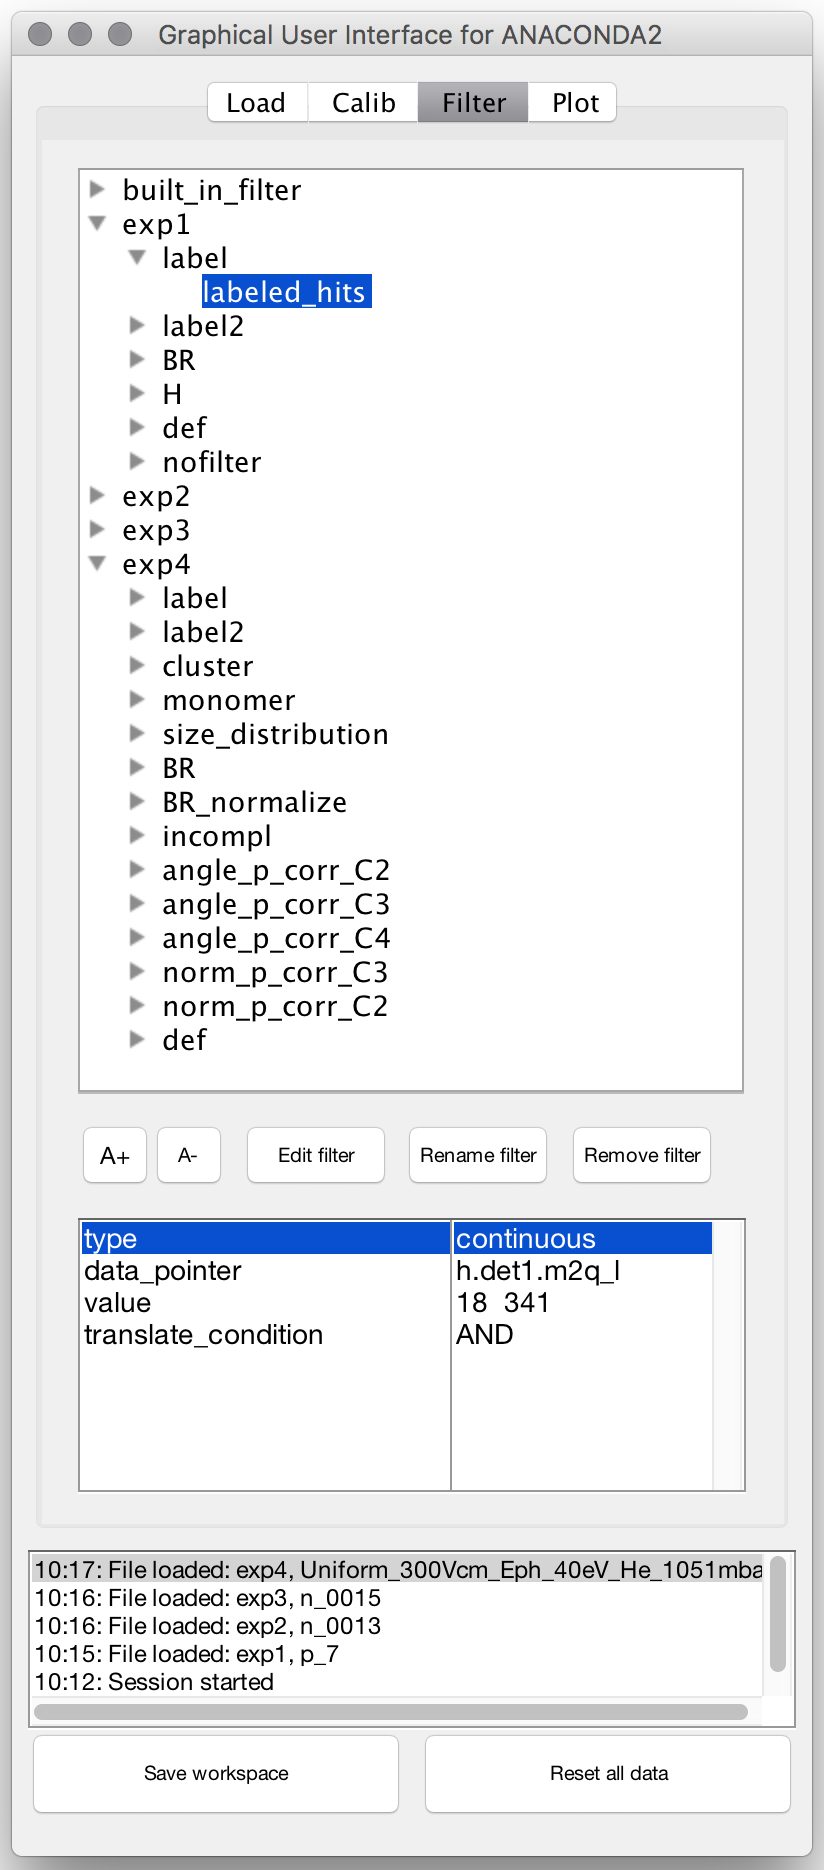
\includegraphics[width=0.34\textwidth]{3_1_filter_sel}
 \caption{The filter tab.}\label{3_1_filter_sel}
\end{wrapfigure}
\\
By opening up the tree of data filters for the different experiments, selecting a filter results in that all its conditions will be shown. If a combined filter is selected, the operator of the combined filter will be shown. If no operator has been defined, the standard condition 'AND' will be shown as operator. To edit a field, double-click on the field to edit, which opens up a window with the previous value (Figure~\ref{3_2_filter_cond_edit}) that can be edited and stored by pressing 'Ok'.\\
\\
Filters can also be combined such that the combined filter consists of one or many hits and/or events filters. A combined filter can also consist of other combined filters. The combined filter(s) then needs an operator that defines how the combined filters will work. The operators that can be selected from are 'AND', 'OR', 'XOR', 'HIT1' and 'HIT2'.\\
\\
As an example, the 'AND'-operator states that all filters that make up the combined filter have to be fulfilled, whilst the 'OR' operator states that at least one filter that is part of the combined filter has to be fulfilled in order to let the event and/or the hit through. The full specification of the filter operators can be found in the main documentation of ANACONDA2 \cite{Bart_Documentation}.\\
\\
To construct a new filter, select one of the built-in filters or the built-in combined filter, and drag-and-drop it to the desired experiment. The parameters can then be edited. Note that filters can also be drag-and-dropped between different experiments.\\
\\
To rename a filter, press the 'Rename' button and type in the desired name. Note that the name has to start with a letter, and there cannot be any spaces or blanks - in these cases, use the underscore symbol.\\
\begin{figure}[h]
\centering
  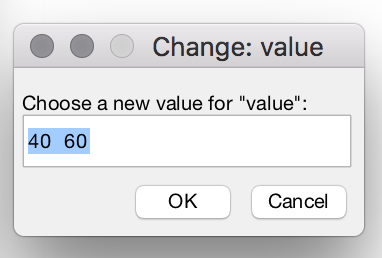
\includegraphics[width=0.3\textwidth]{3_2_filter_cond_edit}
 \caption{The 'Value' of the 'labeled\_hits' filter ie being edited.}\label{3_2_filter_cond_edit}
\end{figure}\\
\begin{figure}[h]
\centering
  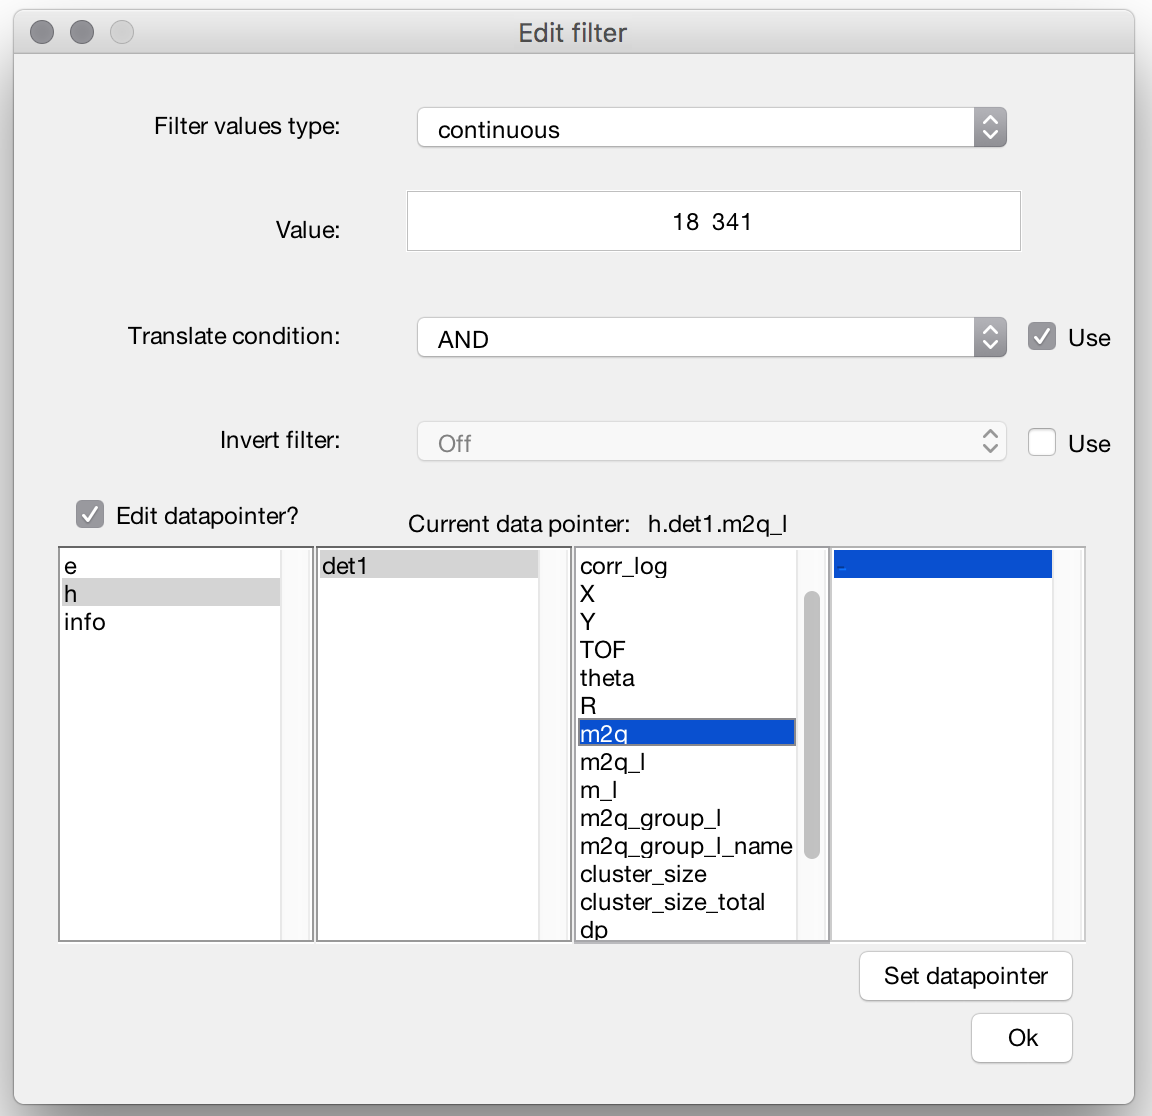
\includegraphics[width=0.8\textwidth]{3_3_filter_edit}
 \caption{Edit all fields of a filter by opening up the 'Edit filter' window.}\label{3_3_filter_edit}
\end{figure}
To fully edit all conditions of a (single, not combined) filter, select a filter and press the edit button. This results in that the 'Edit filter'-window will open up for the selected filter (Figure~\ref{3_3_filter_edit}), in which the filter value type can be selected, the values can be defined, translate condition can be defined or turned on or off, invert filter can be turned on or off, and data-pointer can be edited.\\
\\
A data-pointer defines the 'real' value of raw data, i.e. it points towards a real value (e.g. 'KER' (Kinetic Energy Release)). This is also known as a signal. Since the data-pointer 'points' towards a signal, the edit feature of the data pointer has been constructed such that the user can select signal that the data pointer points towards by using pre-defined signals in the 'Edit filter' window.\footnote{More advanced users can have it completely editable as a text string by double-clicking the data-pointer field without opening the 'Edit filter' window, e.g. for a mathematical formula (e.g. "exp.h.det1.KER/3").}

\clearpage
\section{Data treatment part 4: Plotting}
The last part of data treatment is to plot the data, which can be done by using the plot section under the Plot tab in the GUI. The plot tab has 3 'sub-tabs', as can be seen in Figure~\ref{4_6_plot_tabs}: Pre-defined plots, New plot conf(igurations), and New signal conf(igurations).\\
\begin{figure}[h]
\centering
  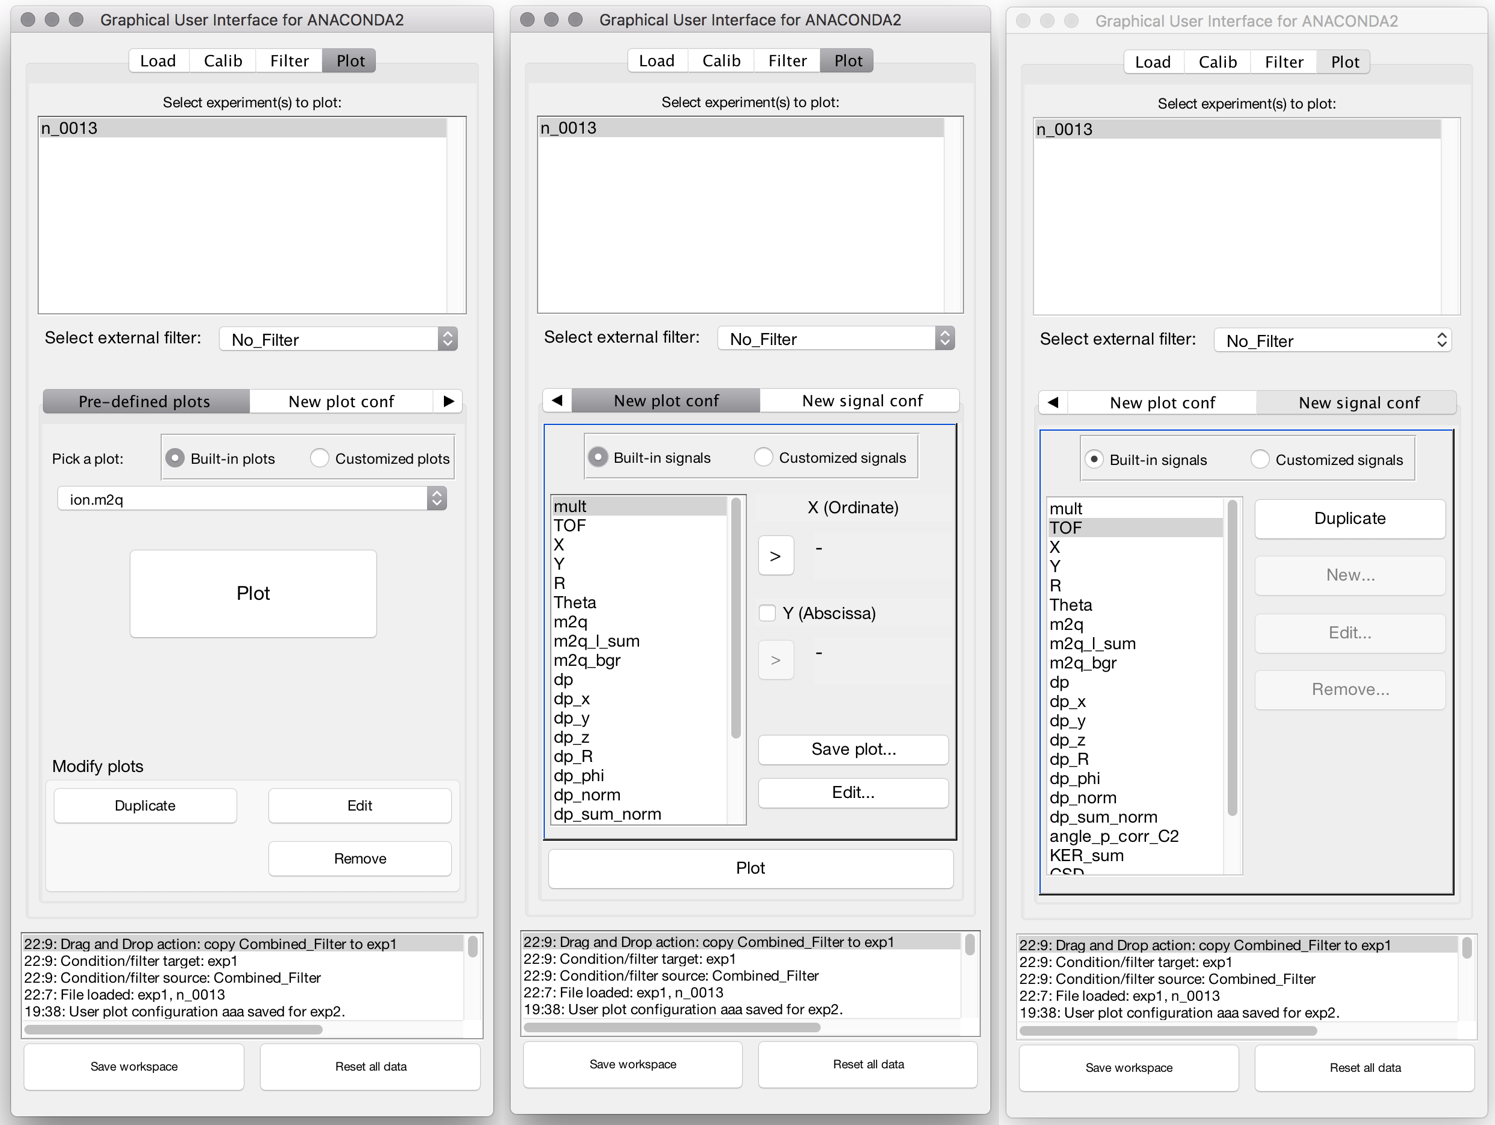
\includegraphics[width=0.9\textwidth]{4_6_plot_tabs}
 \caption{Plot tab's 3 sub-tabs: Pre-defined plots, New plot conf(igurations), and New signal conf(igurations).}\label{4_6_plot_tabs}
\end{figure}\\
In the first sub-tab, i.e. 'Pre-defined plots', the plot configurations are already set and are ready to be plotted by selecting the desired plot configuration and hitting the 'Plot' button. The second sub-tab, i.e. \\
\\
In order for data to be plotted, the signal(s) to be plotted and its (or their) associated metadata have to be defined, as well as their (if any) internal filters and if chosen, an external filter.
\\
We will now go through how to plot the data by using the GUI. The first step is always to select the experiments which are to be plotted by clicking in it/them (multi-selection is available by holding the shift-key whilst clicking on experiments).\\
\\
The fastest way to look at some results is by selecting a built-in plot, which are shown when the radio-button set on 'built-in plots'. One can select to use an external filter or not, and then simply plot the data by pressing the plot button (left window in Figure~\ref{4_6_plot_tabs}).\\
\\
The 'pre-defined plots' sub-tab gives access to two different lists: Built-in and customized plot configurations. The built-in plots are hard-coded and loaded as standard plot types with the experiment during load, whilst the customized plots are the plots that have been constructed by the user in 'New plot conf' sub-tab. The 'New plot conf' and the 'New signal conf' sub-tabs also give access to two different lists: Built-in and customized signals. New signals can be constructed whilst customized signals can be edited and removed in the 'New signal conf' sub-tab, and new plot configurations can be constructed in the 'New plot conf' sub-tab. We will now walk through the whole process, from constructing a new signal and using the new signal to construct a new plot configuration, followed by plotting this and see if we need to do some further editing of the plot configuration.

\subsection{Constructing a new signal}
A new signal can be constructed in two ways: Selecting a previously existing signal (built-in or customized) and pressing duplicate. If the previously existing signal that is to be duplicated was customized, an input dialogue will prompt the user for a new name on the duplicate of the customized signal. If the previously existing signal was built-in, it will be copied to customized signal. The other way to construct a new signal is to select the radiobutton 'Customized signals' and then pressing the button 'New...'. We will go through an example of how to construct a new signal by first duplicating and then editing the duplicated signal.\\
\\
Open the 'New signal conf' tab and ensure that the built-in signals' radio-button is selected, since so far we have not constructed any new signals, i.e. the customized signals list is empty. Then select a signal, which in our case is 'TOF' (time-of-flight). We will, for the construction of the new signal example, refer to Figure~\ref{4_7_dupl_new_signal}'s different numbering, in which each action has been numbered as a sequence for the construction of our new signal.
\\
When the signal (in our case, 'TOF') has been selected, press 'Duplicate' (1). This copies the selected (TOF-) signal to the user-defined signals, which can be found under 'Customized signals'. Select the 'Customized signals' radio-button (2), select the duplicated signal ('TOF') in the signals list and press the 'Edit...' button. This opens the dialog window 'edit signal'. This window can also be reached by pressing the 'New...' button, with the difference that all the value of the fields 'Name', 'Range', 'Binsize', 'Data pointer' and 'Axis label' are empty.\\
\\
We begin by editing the name, bin-size and axis label (4) to the values shown in Figure~\ref{4_7_dupl_new_signal}, marked by an arrow and a '4' above (bottom-left corner window). We then want to look at m2q (mass over charge) rather than TOF. We can switch by choosing a new data pointer that points towards m2q, which we can either do by editing directly in the data pointer's value field or by using the 'Data pointer selector', of which we will do the latter.\\
\\
Since m2q is a hits property, we select 'h' in Listbox 1 (5), which then shows the possible subfields in Listbox 2. In our case, 'h' has only one subfield, i.e. only one detector 'det1', and which we thus select (6). This opens up all subfields that can be used for our detector in Listbox 3, where we see and select 'm2q' (7). Since 'm2q' has no subfields, nothing can be shown in Listbox 4 (which hence remains empty). This enables the 'Set datapointer' button, which we press (8). This changes the value of the field 'Data pointer'.\\
\\
Note that if the selected field in listbox 3 would have a subfield, it would show up in listbox 4. If the selected field in listbox 4 would also have a subfield, all lists would be moved one step to the left. Selecting any field in listbox 1 then resets the data pointer selector.\\
\\
We finish by pressing the 'Ok' button (9) and see that the name has changed in the list of customized signals (since we chose to edit its name).

\begin{figure}[p]
\centering
  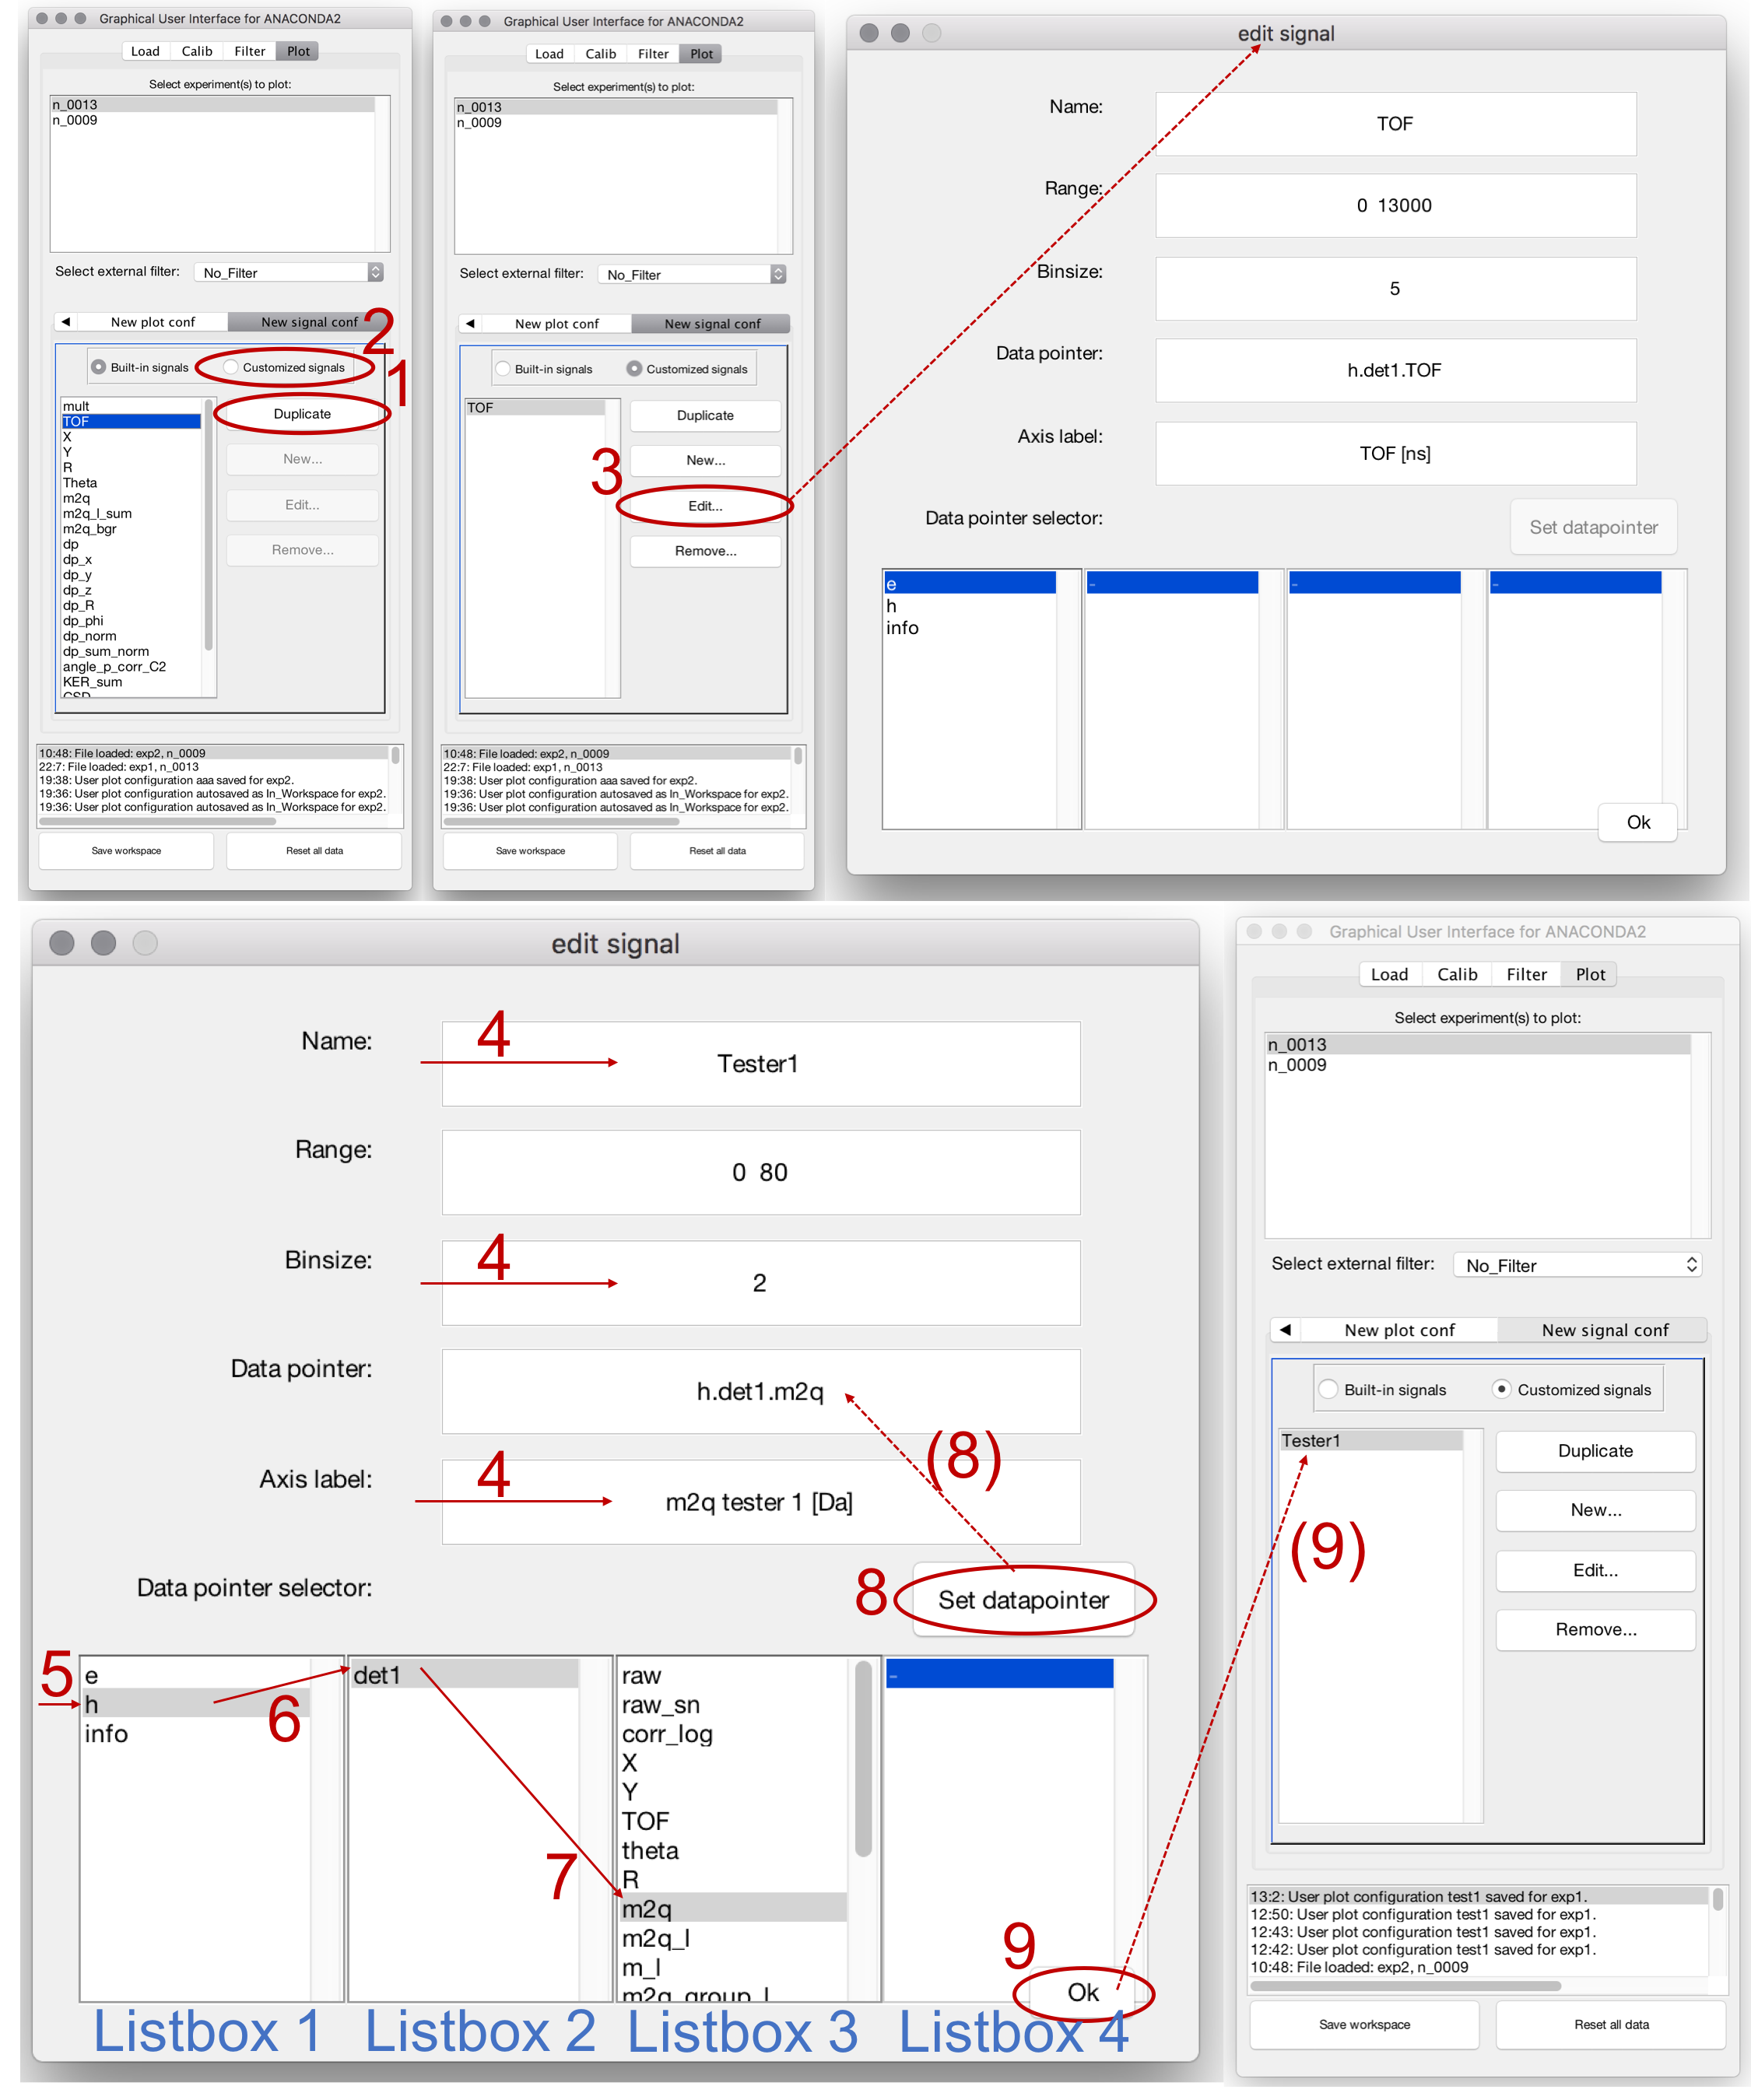
\includegraphics[width=\textwidth]{4_7_dupl_new_signal}
 \caption{Constructing a new signal by duplication followed by editing.}\label{4_7_dupl_new_signal}
\end{figure}

\clearpage
\subsection{Constructing a new plot configuration}
In order to construct a new plot configuration, open the 'New plot conf' sub-tab, select a signal and put it as Ordinate ('X') and/or Abscissa ('Y'). There are many possible combinations between different signals in order to construct a plot configuration out of them. Note that in order to have intensity as abscissa, the check-box for 'Y (Abscissa)' has to be un-checked, and to use something else than intensity as abscissa, click the checkbox so that it is checked. As an example, we will create a new plot configuration with our new signal ('Tester1') as ordinate and a built-in signal ('Theta') as abscissa.\\
\\
We want to use the user-defined (customized) signal ('Tester1') as ordinate. Hence, ensure that the built-in signals' radio-button is selected. Once selected, the user-defined signals will show in the signals listbox. We will, for the construction of the new plot configuration example, refer to Figure~\ref{4_4_new_plotconf}'s different numbering, in which each action has been numbered as a sequence for the new plot conf. construction.\\
\\
When the customized signal for ordinate ('Tester1') has been selected, press the set signal [ $>$ ] (1 in Figure~\ref{4_4_new_plotconf}) to set it as ordinate. Then click to check the abscissa checkbox (2), and open the list of built-in signals (3). Select the signal to be used as abscissa ('Theta') and press the set signal (4) to set it as abscissa. Save the plot configuration (5), write the name of the new plot configuration (6) - which we call 'Testplot1' - and press the 'Ok' button (7). Then switch over to the Pre-defined plots (8) and ensure that the radio-button 'customized plots' (9) is selected. Then open the popup-box with the customized plots (10) and select the constructed plot configuration ('ion.Testplot1'). Note that the plot configurations are named as detector-type ('ion'), followed by a separator (a dot) and plot configuration name ('Testplot'). In order to plot with the saved and customized plot configuration, press the plot button (11). In our case, it generated Figure~\ref{4_8_bad_plot}. The plot seems to be empty due to bad signal values when we constructed our signal ('Tester1'). We will walk through the process of editing a plot configuration in the variable editor in section 5.3.\\
\\
The plot configuration can also be used for plotting the experiment without saving. One way is to press the plot button directly (X in Figure~\ref{4_4_new_plotconf}) in the 'New plot conf' sub-tab (instead of in the pre-defined plots' sub-tab). The other way is to select the 'In\_Workspace' plot configuration in the popup-box with the customized plots (10) in the pre-defined plots' sub-tab, which is also defined by its detector specie ('ion'). The saved (customized) plot configurations can be edited and removed by first being selected (10) and then pressing the edit/remove button.

\begin{figure}[p]
\centering
  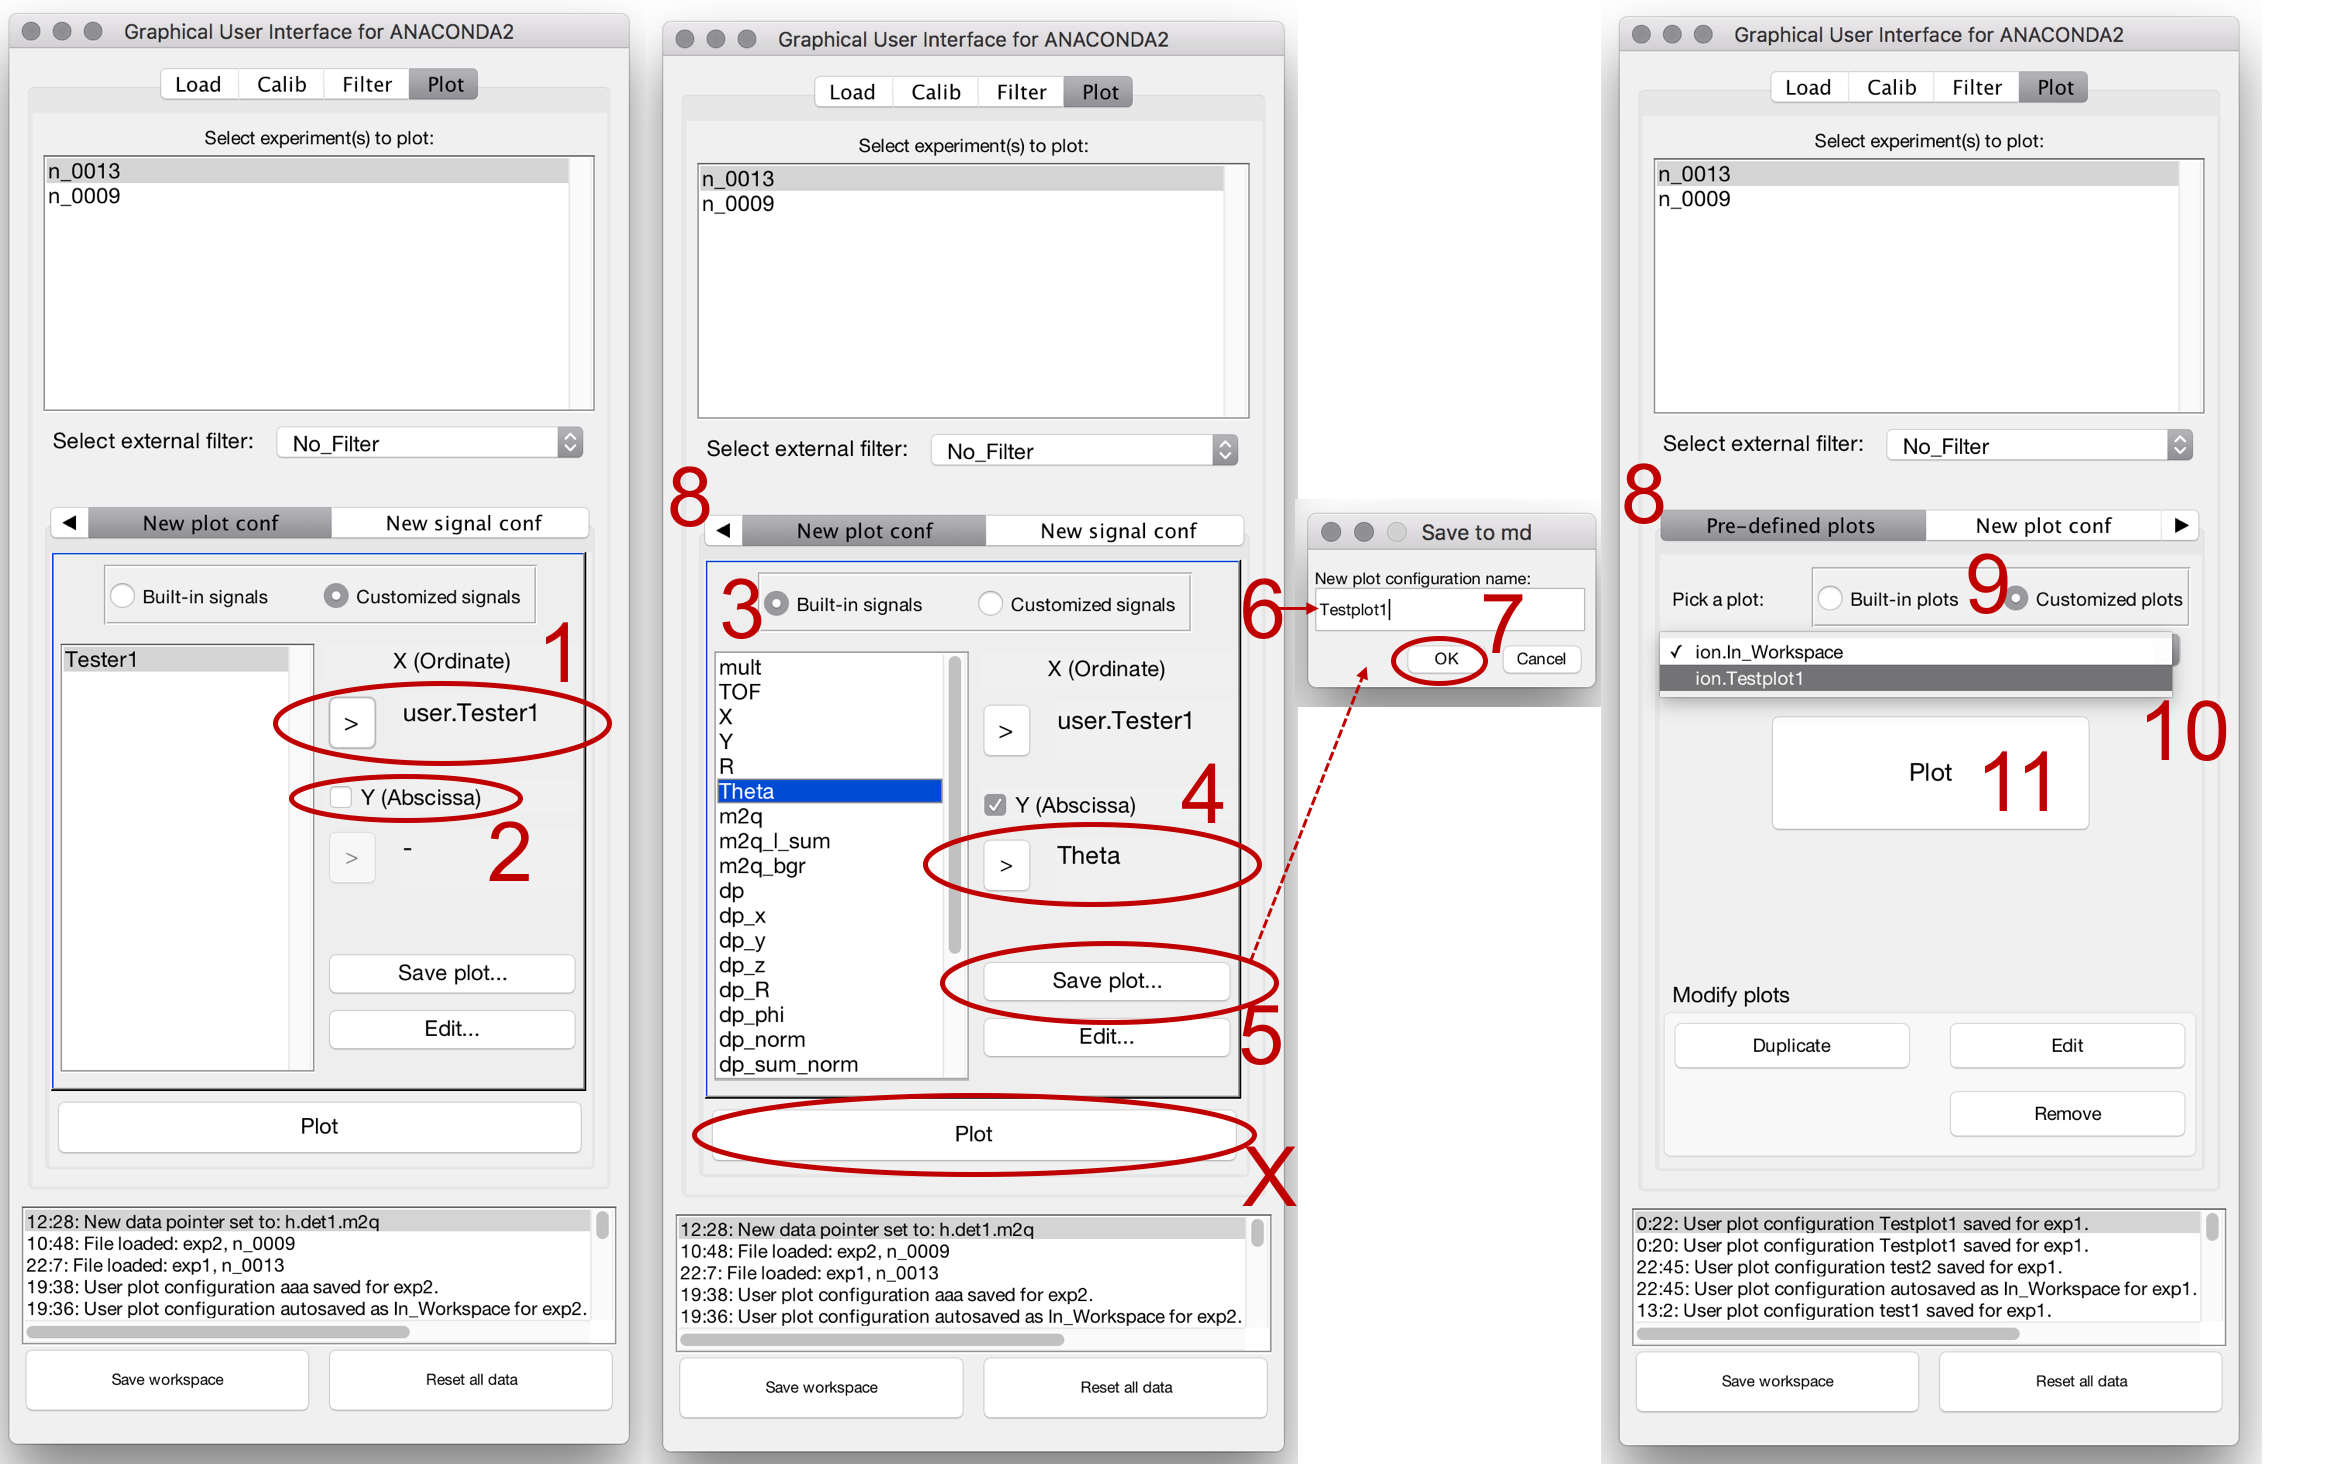
\includegraphics[width=\textwidth]{4_4_new_plotconf}
 \caption{Constructing a new plot configuration from the previously constructed (customized) signal 'Tester1' as ordinate and the built-in signal 'Theta' as abscissa.}\label{4_4_new_plotconf}
\end{figure}

\begin{figure}[p]
\centering
  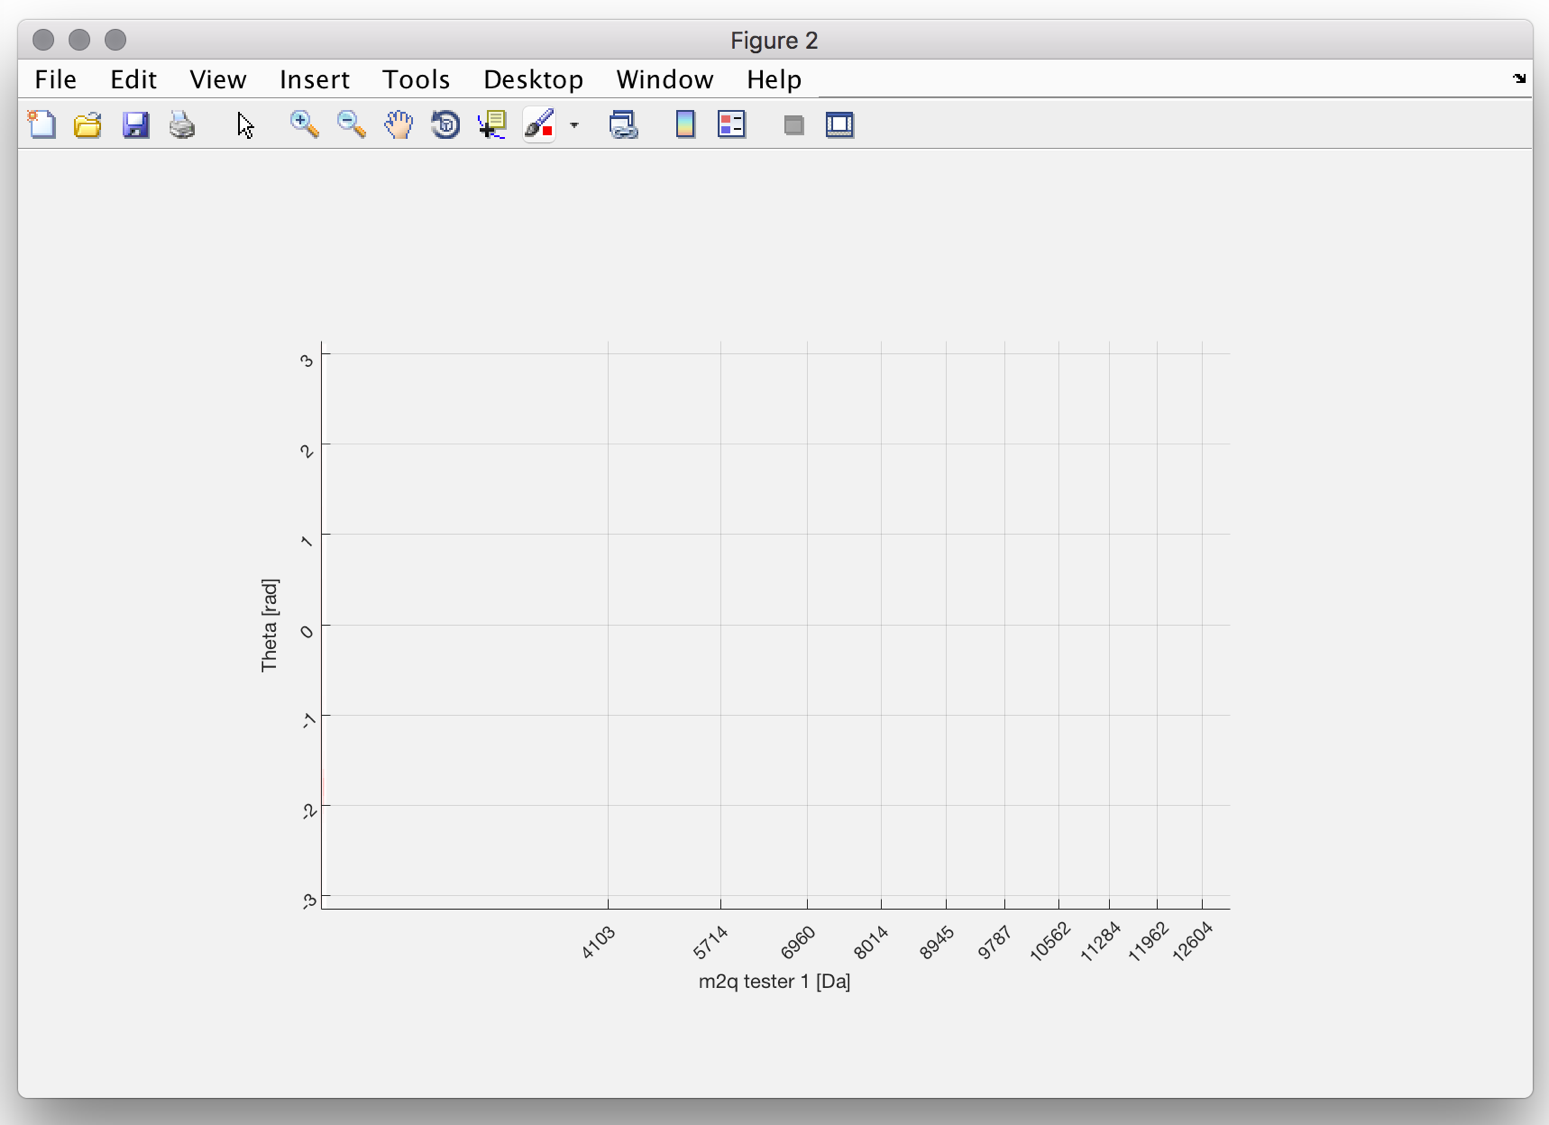
\includegraphics[width=0.5\textwidth]{4_8_bad_plot}
 \caption{The resulting plot from the process described above, with the customized 'Tester1' signal on the x-axis and the built-in 'Theta' signal on the y-axis.}\label{4_8_bad_plot}
\end{figure}

\clearpage
\subsection{Editing with the variable editor}
As can be seen in Figure~\ref{4_8_bad_plot}, the plot seems to be empty. This is probably due to that something is 'bad' with at least one of the signals used as the plot configuration, of which our signal ('Tester1) is probably the cause. Hence, we will look into it with the variable editor.\\
\\
In order to open the variable editor, we select the customized plot ('Testplot1') in the popup-box with the customized plots in the sub-tab 'Pre-defined plots' and then press the 'Edit' button. This opens up the variable editor in the main MATLAB window ('Variables - md\_GUI.mdata\_n.exp\#.plot.user.det1.Testplot1'), as can be seen in Figure~\ref{4_9_variable_editor}. In the variable editor, we see 4 structures: Figure (which contains information about the plot container, such as color, position and size), axes (which contains information about the x- and y-axis, such as limits, ticks, tick-labels, labels, etc.), hist (histogram, which contains information about the plot data, such as bin-size, range, number of dimensions and data-pointers) and GraphObj (graphical object properties, such as image type, marker type, marker edge color, etc.).\\
\\
Since we cannot see anything in Figure~\ref{4_8_bad_plot}, we make an initial guess that this problem is caused by the axes. We hence open up the axes structure by double-clicking it, resulting in that a new tab is opened up in the variable editor window (Figure~\ref{4_10_variable_editor_axes}). We investigate the XTicks by double-clicking it and find values from 4103 to 17791. This would mean very large masses, but these values come from that we previously duplicated a time-of-flight signal with time units instead of mass-over-charge units. Hence, we change those to values we know will show up for the loaded experiment, which happens to be carried out on pyridine and pyridine fragments. We also change the XTickLabel to show the name of the fragments they are associated with, as described in the Table \ref{XTicks} below, and the XLim values from 0 to 80. 
\begin{center}
Table \ref{XTicks}: X ticks and X tick labels, i.e. molecules and their mass-over-charge.\\
\begin{tabular}{ c c c }
\\ \hline
$XTickLabel$ & $XTick value$\\
\hline
H$^+$			&	1	\\
C$^+$			&	12	\\
C$_2^+$			&	24	\\
C$_3^+$			&	36	\\
C$_4^+$			&	48	\\
C$_5$H$_5$N$^+$	&	79	\\
\hline
\label{XTicks}
\end{tabular}
\end{center}
\begin{figure}[h]
\centering
  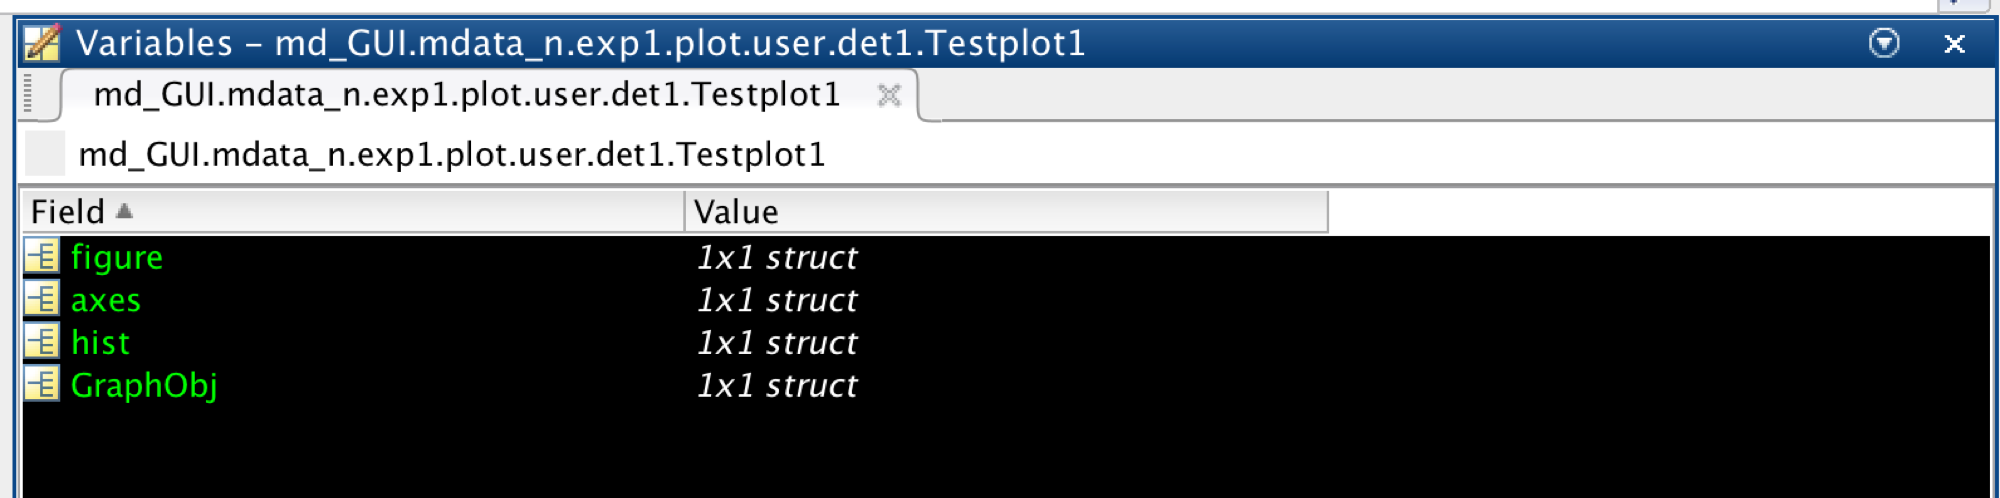
\includegraphics[width=0.8\textwidth]{4_9_variable_editor}
 \caption{Variable editor for the Testplot1 .}\label{4_9_variable_editor}
\end{figure}
\begin{figure}[h]
\centering
  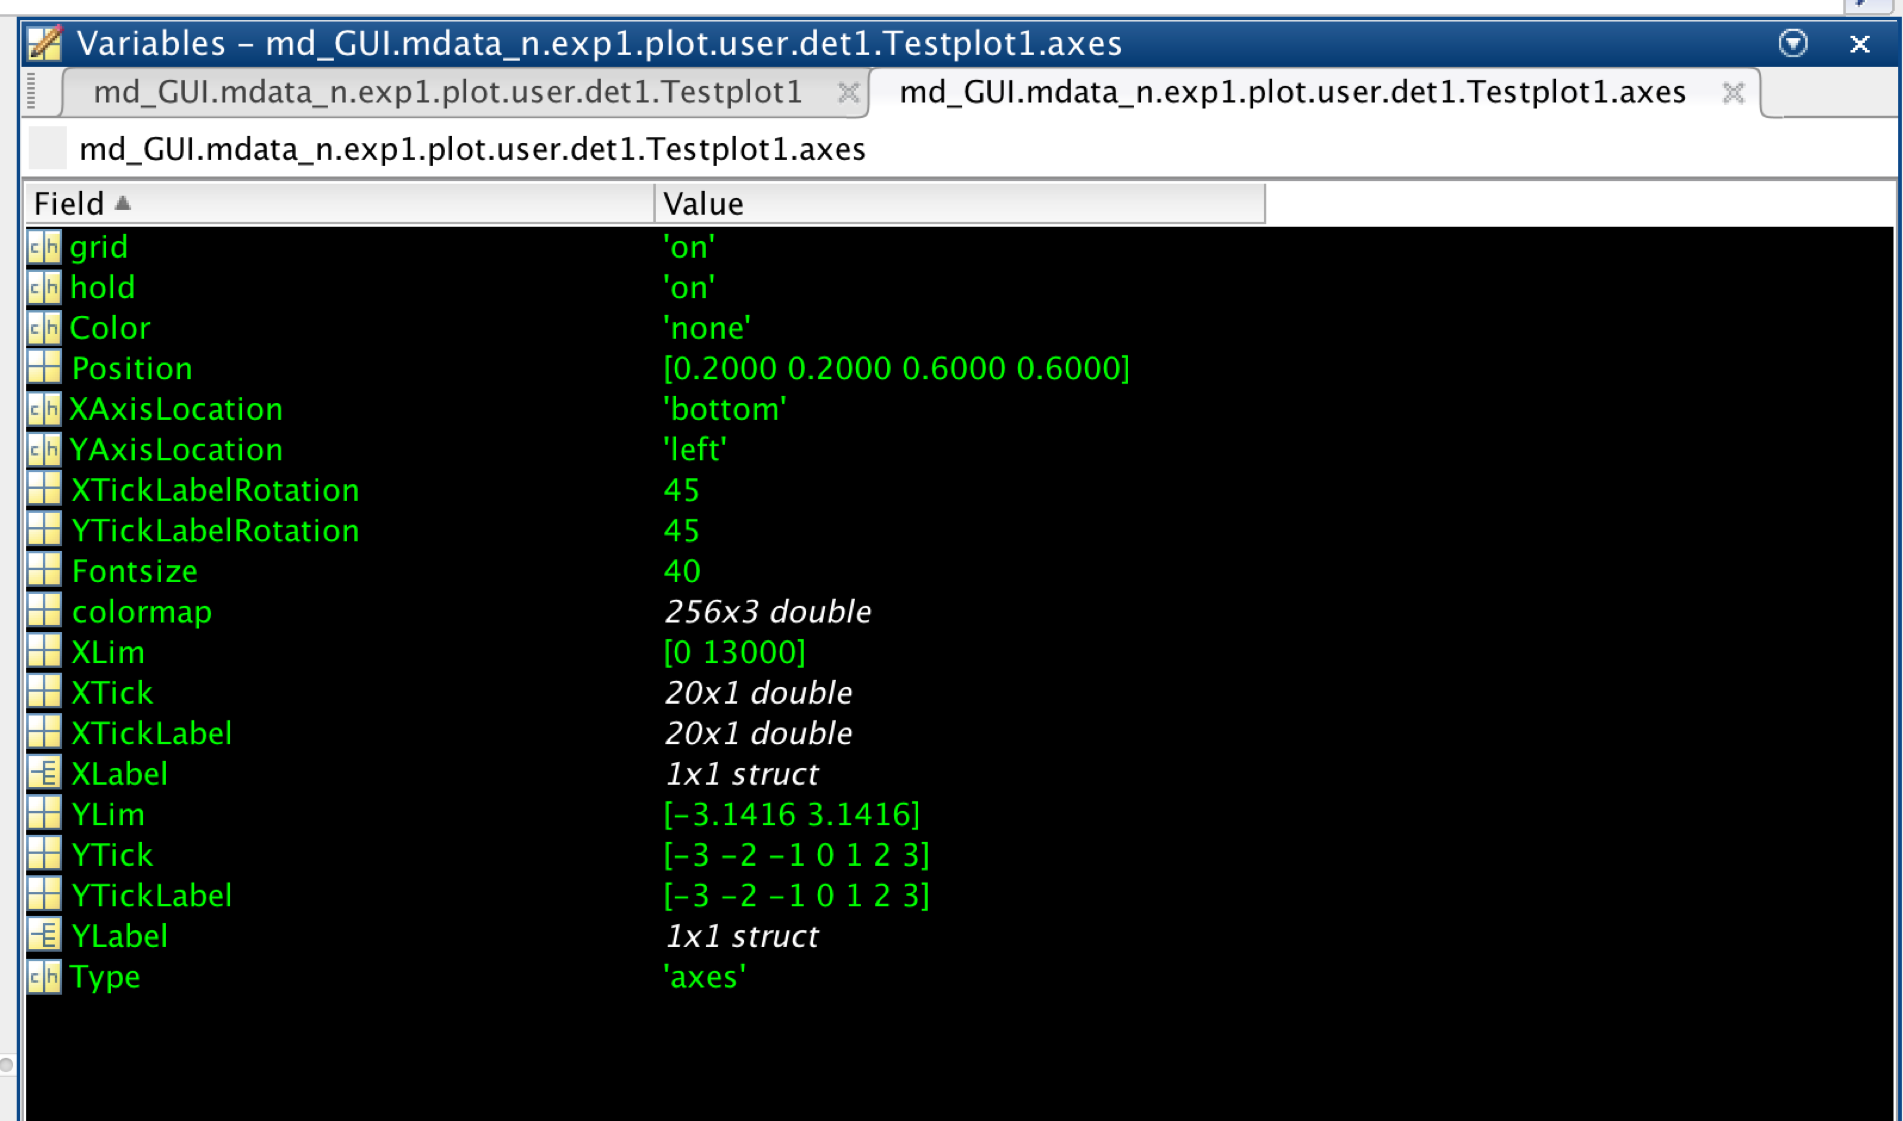
\includegraphics[width=0.8\textwidth]{4_10_variable_editor_axes}
 \caption{Variable editor for Testplot1's axes properties.}\label{4_10_variable_editor_axes}
\end{figure}
When we plot this plot configuration, the result is Figure~\ref{4_11_newplot_badbin}. We notice that the bin-sizes seem to be too large in the x-direction, so we edit the close the variable editor for the axes and open the variable editor for the histograms by double-clicking on the hist structure, and then on the bin-size. We change the value of the first column from 2 to 0.5, and then we plot the plot configuration again. This results in Figure~\ref{4_12_newplot_goodbin} when we plot this plot configuration. 
\clearpage
\begin{figure}[p]
\centering
  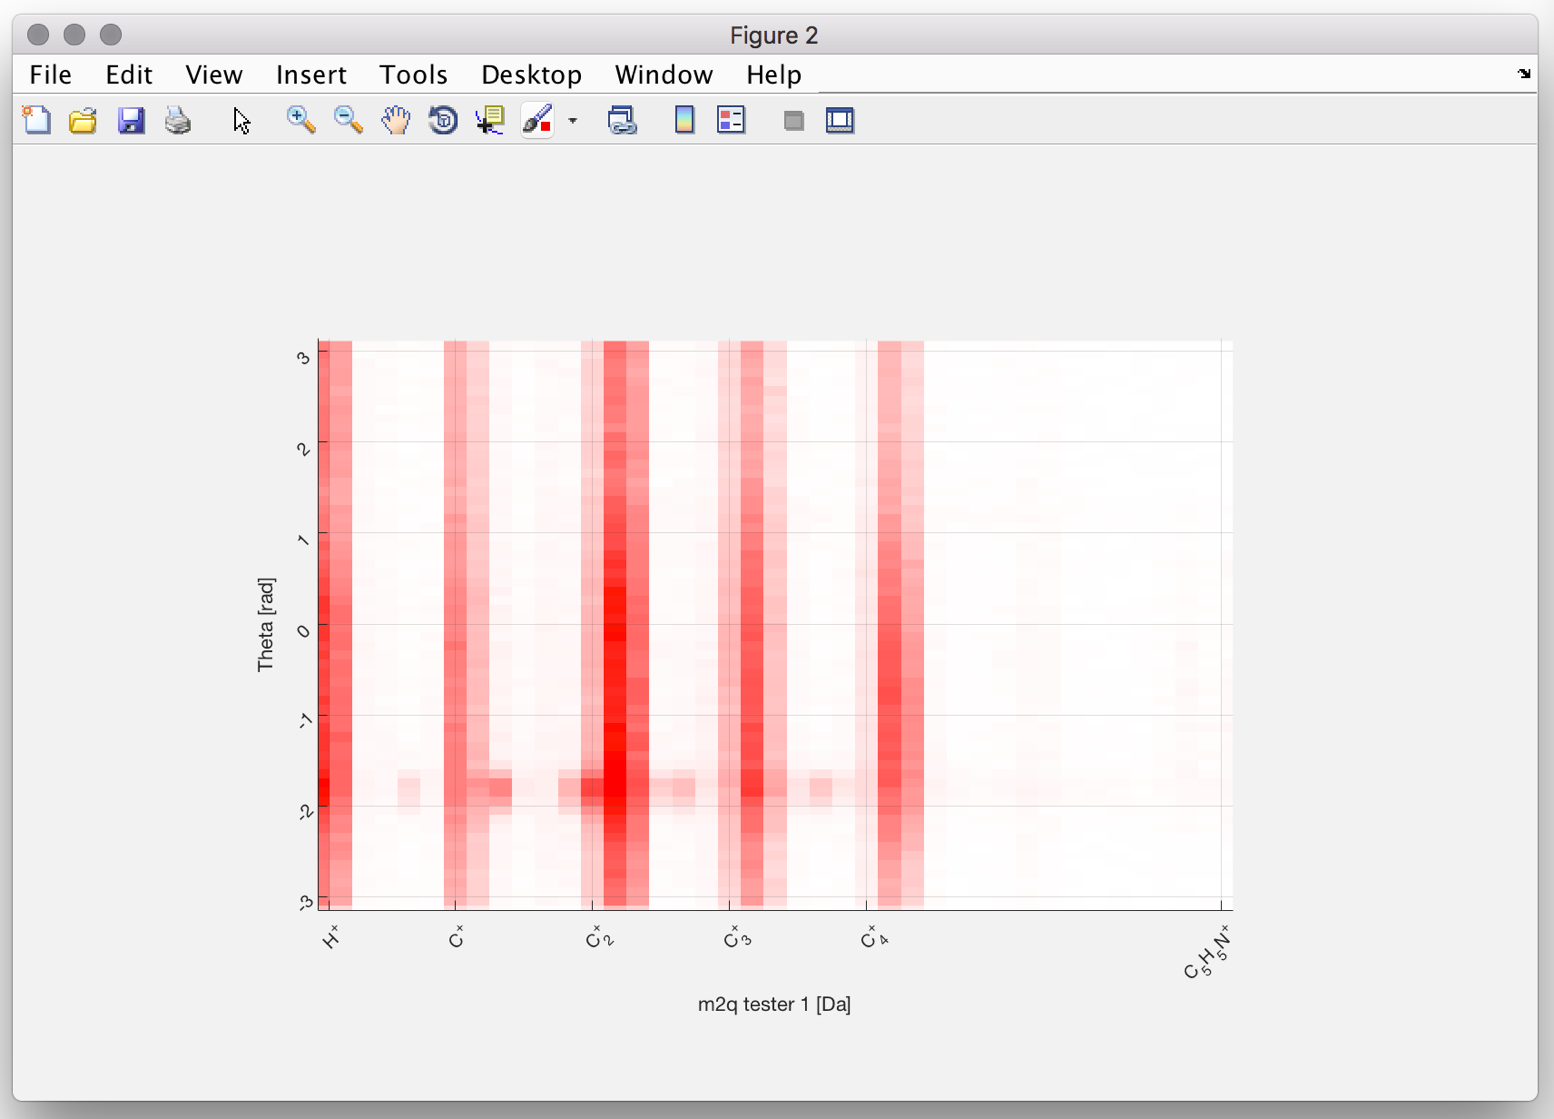
\includegraphics[width=0.75\textwidth]{4_11_newplot_badbin}
 \caption{Our signal in units mass over charge plotted against theta.}\label{4_11_newplot_badbin}
\end{figure}
\begin{figure}[p]
\centering
  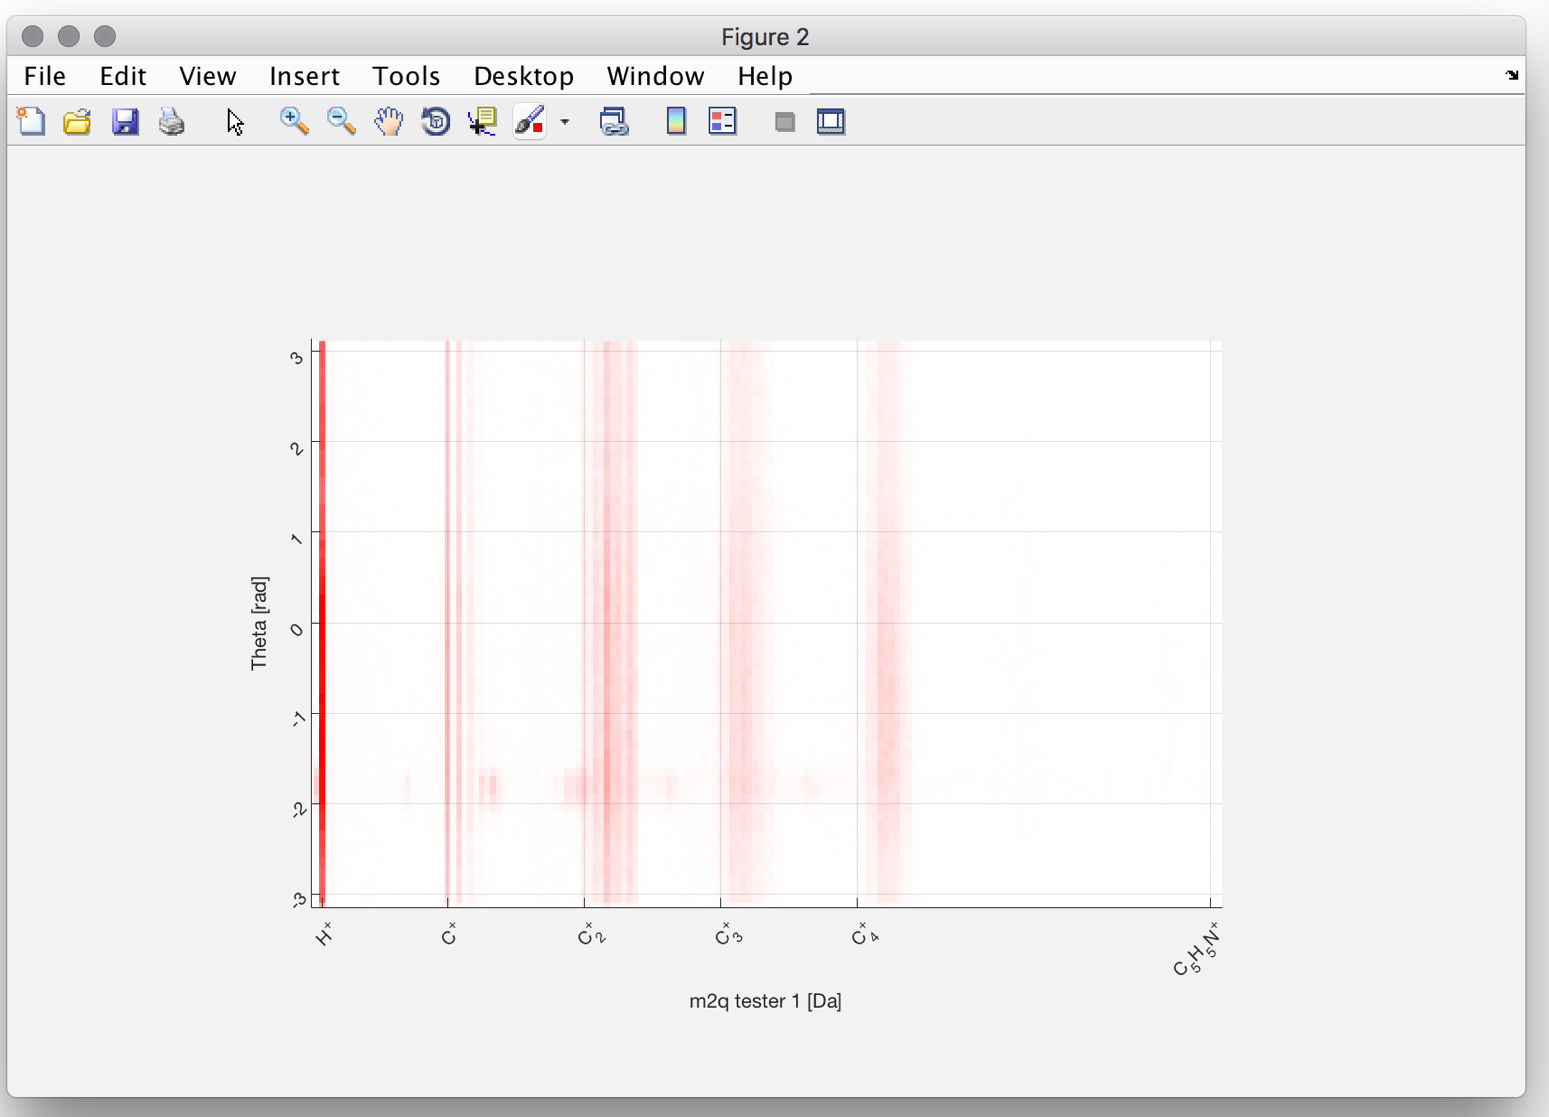
\includegraphics[width=0.75\textwidth]{4_12_newplot_goodbin}
 \caption{Our signal in units mass over charge plotted against theta after correcting the bin-size of our signal from bin-size 2 to bin-size 0.5.}\label{4_12_newplot_goodbin}
\end{figure}

\clearpage
\section{Data treatment part 5: Plot data selection}
The data process schematics for plotting has been illustrated in Figure~\ref{4_5_internal_plot_process}, when the plotting has started, the GUI first checks if a filter has been selected. If no, the internal filters (if any) will be used, and if yes, the selected filter will be used and then (in this version) overwrites the built-in filter. This becomes part of the experiment MetaData, which together with the selected signal(s) are plotted by the software in the way it was defined by the user in the plot configurations.
\begin{figure}[h]
\centering
  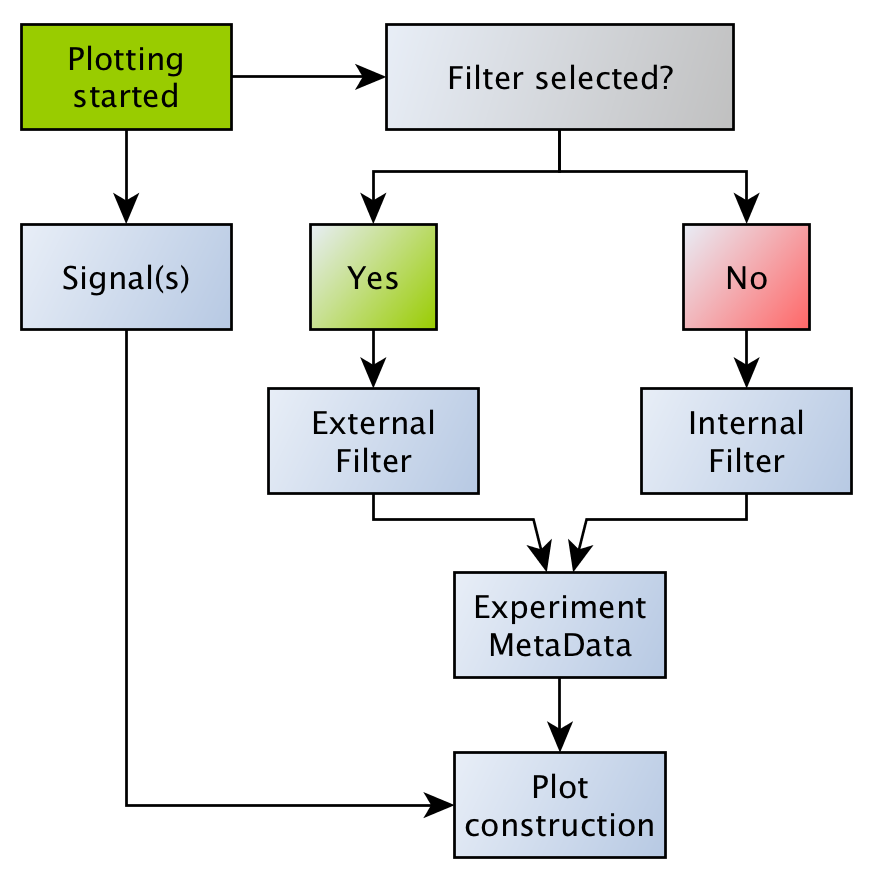
\includegraphics[width=0.5\textwidth]{4_5_internal_plot_process}
 \caption{Plot process data flow schematics.}\label{4_5_internal_plot_process}
\end{figure}\\
In order to demonstrate how data can be selected by using various data filters, the same experiment's PEPIPICO (photo-excitation photo-ionization photo-ionization coincidence) map (m2q for HIT1 and HIT2) will be plotted three times; once without any filters applied and twice with filters applied. First we use no filter to look at the entire map in Figure~\ref{4_13_Filters}, whilst the second time we want to look at only 2 specific events (in the same plot): A kinematically incomplete detection (No. 1) and a(n) (almost) kinematically complete detection (No. 2). The third time we look at only one event, which is a kinematically complete detection (No. 3).\\
\\
The experiment we analyze was carried out at MAXLAB in 2011; pyridine studied with synchrotron radiation. In the analyzed experimental data, the energy of the photons was 399.1eV.\\
\\
No. 1: For the kinematically incomplete detection we want to observe the channels corresponding to N$^+$ (HIT1, m2q = 14) with C$_3$H$^+$ (HIT2, m2q = 37), which together corresponds to a detection of C$_3$H$^{++}$N and hence, a total loss of 2C and 4H. For this, we construct a combined filter with a hits condition: $13.5 < m2q < 14.5$, and an events condition: $50.5 < m2q < 51.5$. This combined filter will be named 'FiltNo1' and have an 'AND' operator, see Figure~\ref{4_13_Filters}E.\\
\\
No. 2: For the (almost) kinematically complete detection we want to observe the channels corresponding to CN$^+$ (HIT1, m2q = 26) with C$_4$H$^+$ (HIT2, m2q = 49), which together corresponds to a detection of C$_5$H$^{++}$N and hence, a total loss of 4H. For this, we construct a combined filter with a hits condition: $25.5 < m2q < 26.5$, and an events condition: $74.5 < m2q < 75.5$. This combined filter will be named 'FiltNo2' and have an 'AND' operator, see Figure~\ref{4_13_Filters}F.\\
\begin{wrapfigure}{r}{0.33\textwidth}
\centering
  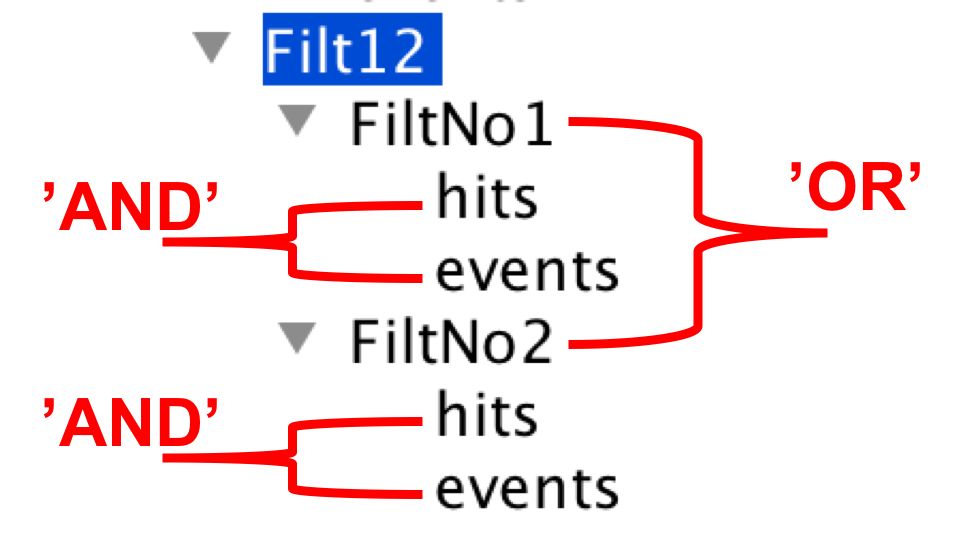
\includegraphics[width=0.33\textwidth]{4_14_doublecomb_filt}
 \caption{A two-level combined filter: Filt12 consists of the two combined filters FiltNo1 and FiltNo2, of which each consists of a hits-filter and an events-filter.}\label{4_14_doublecomb_filt}
\end{wrapfigure}\\
No. 3: For the kinematically complete detection we want to observe the channels corresponding to CHN$^+$ (HIT1, m2q = 27) with C$_4$H$_4^+$ (HIT2, m2q = 52), which together corresponds to a detection of C$_5$H$_5^{++}$N and hence, no loss. For this, we construct a combined filter with a hits condition: $26.5 < m2q < 27.5$, and an events condition: $78.5 < m2q < 79.5$. This combined filter will be named 'FiltNo3' and have an 'AND' operator, see Figure~\ref{4_13_Filters}B,C.\\
\\
For plotting No. 1 and No. 2 together in a single plot, we have to combine their filter conditions, which we name 'FiltNo12'. This means that we combine two combined filters with an 'OR' operator, see Figure~\ref{4_13_Filters}D and Figure~\ref{4_14_doublecomb_filt}.

\clearpage
\begin{figure}[p]
\centering
  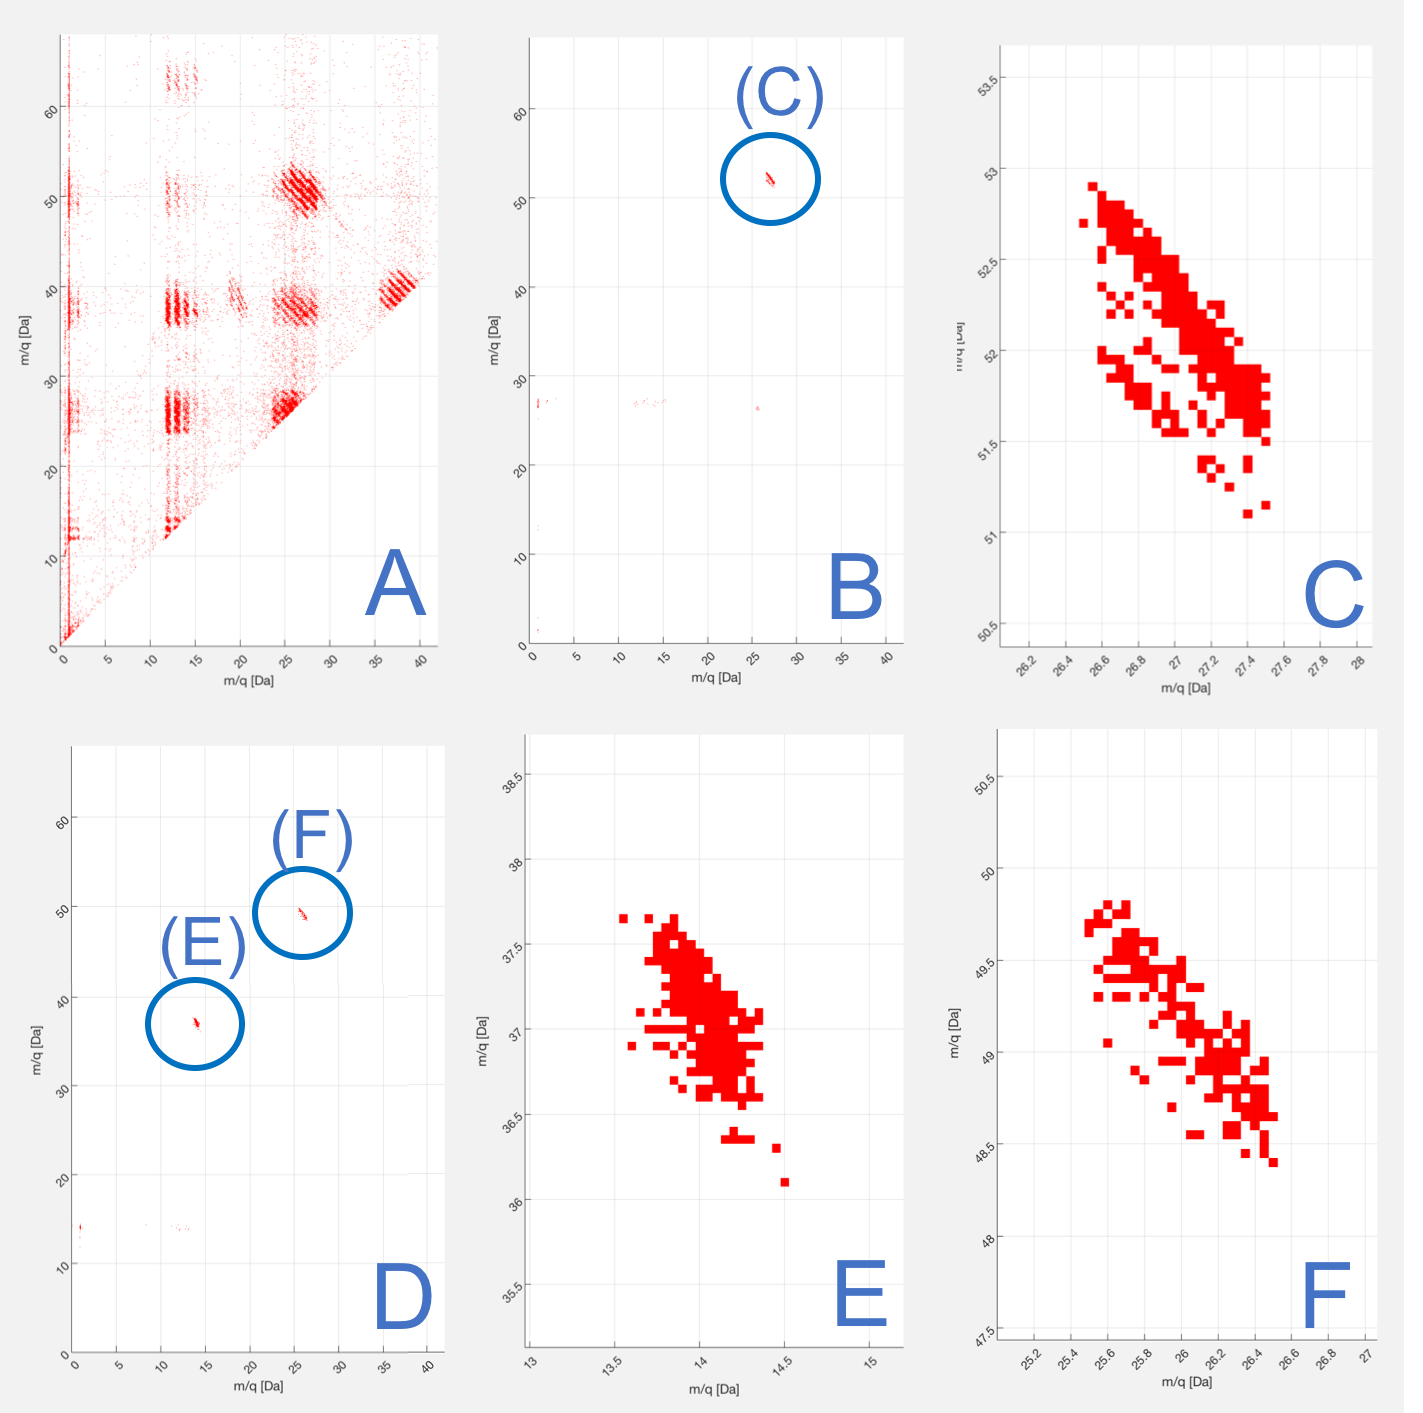
\includegraphics[width=\textwidth]{4_13_Filters}
 \caption{A PEPIPICO plot for an ion-ion coincidence experiment with pyridine.}\label{4_13_Filters}
\end{figure}

\clearpage
\section{Experiment 1: Pyridine molecules}
- - -

\clearpage
\section{Experiment 2: Pyridine and water clusters}


\clearpage
\section{Experiment 3: Helium}


\clearpage
\section*{Table ...}%%%%%%%%%%
Table showing the meaning of e.g. m2q, m2q\_l

\clearpage
\section*{References}
\begin{thebibliography}{9}

\bibitem{Bart_Documentation}
  Bart Oostenrijk,
  \textit{Description of the Coincidence data analysis software},
  Department of Physics at Lund University,
  2nd edition,
  2018.

\end{thebibliography}
 - Joakim Laksman phd\\

\end{document}


























